%%%%%%%%%%%%%%%%%%%%%%%%%%%%%%%%%%%%%%%%%%%%%%%%%%%%%%%%%
%%%%%IMPORTS:
%packages a utilizar:
\documentclass{report}
\usepackage[T1]{fontenc}     % Fontes T1
\usepackage[utf8]{inputenc}  % Input UTF8
\usepackage[top=3cm,bottom=3cm,left=3cm,right=2.5cm,asymmetric]{geometry} %fronteiras
%\usepackage[nottoc]{tocbibind}
\usepackage[table]{xcolor} %Colorir tabelas
\usepackage[backend=biber, style=ieee]{biblatex} %bibliografia
\usepackage{csquotes}  % referências
\usepackage[portuguese]{babel} %Usar língua portuguesa
\usepackage{blindtext} 
\usepackage[printonlyused]{acronym}  %Acrónimos
\usepackage{hyperref}  %Autoref no índice
\usepackage{graphicx}  %Usar imagens
\usepackage{titling}
\usepackage{multicol} %multicoluna de texto
\usepackage{adjustbox}
\renewcommand{\figurename}{Fig.} 
\renewcommand{\tablename}{Tabela} 
\usepackage[font=small,tableposition=top]{caption} 
\usepackage[font=small]{subcaption}
\usepackage{xcolor} %cor nos textos
\usepackage{amsmath} %matematica
\usepackage{amssymb} %simbolos matematicos
\graphicspath{ {./images/} } %directorio das imagens
\usepackage{fancyhdr}
\usepackage{authblk}
\usepackage{float} %Posicionamento exacto das figuras no texto
\usepackage{url}   %referencias URL
\usepackage{blindtext}
\def\UrlBreaks{\do\/\do-} %não cortar referencias

\usepackage{indentfirst} %Garantir avanço do primeiro parágrafo
\hypersetup{pdfborder=0 0 0} %Remover a caixa vermelha das referências
\usepackage{chngcntr} %Numeração contínua das figuras
\counterwithout{figure}{chapter} %Numeração contínua de figuras
\counterwithout{table}{chapter} %Numeração contínnua de tabelas
\setlength{\parskip}{0.2cm} %Aumento de espaçamento entre parágrafos

\usepackage{hyperref}


\begin{document}	
	%Definições do Relatório

%Dados Gerais:
\def\titulo{Projecto Final: \\ Máquina de Lavagem de Roupa}
\def\data{Junho de 2022}
\def\versao{Ver.: 1.13}
\def\departamento{Departamento de Electrónica Telecomunicações e Informática}
\def\empresa{Universidade de Aveiro}
\def\logotipo{logotipo_ua.png}

%Dados dos Autores:
%primeiro autor:
\def\pautor{João Pedro Nunes Vieira} 
\def\numpautor{Nº Mec.:  50458}
\def\contactopautor{joaopvieira@ua.pt}
%segundo autor:
\def\sautor{Leandro Roque Costa} 
\def\numsautor{Nº Mec.: 110326}
\def\contactosautor{lrc@ua.pt}
%
\def\autores{\pautor \\ \sautor}

	%Capa do Relatório:
\begin{titlepage} 
	\begin{center}
	\includegraphics[scale=0.50]{\logotipo}
	\line(1,0){350} \\ 
		\vspace*{2mm}
	{\Large \uc} \\
		\vspace*{2mm} 	
	{\Huge \titulo} \\
		\vspace*{2mm}
	\line(1,0){350} \\ 
		\vspace*{2mm}
	{\Large \empresa} \\
		\vspace*{20mm}
	{\Large \autores} \\ 
		\vspace*{\fill}
	\end{center}

	\begin{flushright} 
		{\large \departamento} \\ 
		{\versao} 
	\end{flushright}

\end{titlepage}

	%Página de Título:
\predate{\begin{flushright}\small}
\postdate{\par\end{flushright}}

\title{ 
	{\huge\textbf{\titulo} } \\ 
	{\large \departamento\\ \empresa} }

\author{

    \begin{tabular}{l}
        \pautor, \numpautor\hfil \\
        \contactopautor
    \end{tabular}
    \and
    \begin{tabular}{l}
        \sautor, \numsautor\hfil \\
        \contactosautor
    \end{tabular}
    \and
    \begin{tabular}{l}
        \tautor, \numtautor\hfil \\
        \contactotautor
    \end{tabular}
    \and
    \begin{tabular}{l}
        \qautor, \numqautor\hfil \\
        \contactoqautor
    \end{tabular}
}




\date{\vspace{\fill}{\data}} 
\maketitle
	\begin{abstract}

O presente relatório aborda a comunicação entre aplicações seguindo um modelo Cliente-Servidor, usando conceitos abordados no decorrer da Unidade Curricular de Laboratórios de Informática, nomeadamente programação de sockets TCP, Criptografia, Documentação JSON, programação em Python, etc... \\
Este trabalho é relevante pois com o avanço tecnológico actual, a aprendizagem dos conceitos anteriormente referidos torna-se imperativa para os estudantes de cursos ligados à tecnologia de informação.\\
O projecto foi realizado por duas pessoas, tendo como objectivo o desenvolvimento das capacidades de trabalho em grupo, desenvolvimento e estruturação de código, realização de testes funcionais e planeamento através da plataforma \textbf{code.ua.pt}. \\
Foi possível implementar com sucesso um modelo de comunicação entre aplicações Cliente-Servidor em gênero "Jogo High-Low" com funcionalidade de segurança(encriptação) de forma simples, prática e eficaz, conseguindo-se corrigir todos os erros encontrados.

\end{abstract}
	
%%%%%%%%%%%%%%%%%%%%%%%%%%%%%%%%%%%%%%%%%%%%%%%%%%%%%%%%%
%%%%%INDICE:

\renewcommand{\contentsname}{Índice}
\tableofcontents
\listoffigures
\pagenumbering{roman}

%%%%%%%%%%%%%%%%%%%%%%%%%%%%%%%%%%%%%%%%%%%%%%%%%%%%%%%%%
%%%%%ACRÓNIMOS:

\chapter*{Acrónimos}
\begin{acronym}

\acro{ua}[UA]{Universidade de Aveiro}
\acro{deti}[DETI]{Departamento de Eletrónica, Telecomunicações e Informática}
\acro{leci}[LECI]{Licenciatura em Engenharia de Computadores e Informática}
\acro{uc}[UC]{Unidade Curricular}
\acro{sio}[SIO]{Segurança Informática e Nas Organizações} 
\acro{cwe}[CWE]{Common Weakness Enumeration}
\acro{cia}[CIA]{Confidenciality, Integrity and Availability}
\acro{pc}[PC]{Personal Computer}
\acro{www}[WWW]{World Wide Web}
\end{acronym}

%%%%%%%%%%%%%%%%%%%%%%%%%%%%%%%%%%%%%%%%%%%%%%%%%%%%%%%%%
%%%%%HEADERS & FOOTERS:

\pagestyle{fancy}
\fancyhf{}
\chead{\titulo}
\cfoot{\thepage}
%%%%%%%%%%%%%%%%%%%%%%%%%%%%%%%%%%%%%%%%%%%%%%%%%%%%%%%%%
%%%%%%%%%%%%%%%%%%%%%%%%%%%%%%%%%%%%%%%%%%%%%%%%%%%%%%%%%
%%%%%INTRODUÇÃO:
%
\chapter{Introdução}
\label{chap.Intro}
\pagenumbering{arabic}

O presente projecto é dedicado ao desenvolvimento de um website no estilo de loja online, concebido com o objectivo de promover e vender merchandise do \acf{deti} da \acf{ua} , incorporando abordagens essenciais da Segurança Informática e aplicando conceitos fundamentais lecionados no presente ano lectivo no decorrer da \acf{uc} de \acf{sio} do curso de \acf{leci}, com especial foco em: 

\begin{enumerate}
	\item Previsibilidade constante do sistema e solução apresentada (estratégia defensiva).
	\item Defesa contra atividades não autorizadas (garantindo o funcionamento seguro e ininterrupto da plataforma).
	\item Conceitos de \acf{cia} da Segurança da Informação.
	\item Conceitos de \acf{cwe}
\end{enumerate}


\section{Enquadramento}
\label{sec.enquadramento}
Com a introdução dos conceitos de \ac{pc} e \ac{www} à sociedade e público geral, foram introduzidos diversos benefícios e desafios de segurança. A dependência dos sistemas digitais complexos é um paradigma da sociedade contemporânea tornando assim imperativa a aprendizagem de conceitos fundamentais relativos à proteção de informações pessoais e confidenciais, e à garantia do funcionamento previsto (e seguro) dos sistemas e soluções digitais apresentadas ao público comum. \\

Este enquadramento destaca a relevância do projeto ao abordar questões cruciais, tais como:

\begin{itemize}
  \item A necessidade de garantir a segurança de sistemas e informações num ambiente digital.
  \item A aplicação prática dos conceitos de \ac{sio} adquiridos.
  \item O compromisso com a proteção dos dados pessoais e/ou confidenciais dos utilizadores.
  \item O desenvolvimento de competências de detecção e prevenção de vulnerabilidades comuns \ac{cwe}.
  \item A realização de análise e auditoria para identificar potenciais falhas, erros e exposições, assim como identificar e avaliar o seu impacto caso seja realizado um ataque com base em cada um destes.
\end{itemize}

%
%%%%%%%%%%%%%%%%%%%%%%%%%%%%%%%%%%%%%%%%%%%%%%%%%%%%%%%%%
%%%%%CAPÍTULO 2: FUNCIONAMENTO PREVISTO 
%
\chapter{Funcionamento Previsto do Website}
\label{chap.Funcionamento}
\pagenumbering{arabic}

\section{Home Page}
\label{sec.home}

Página inicial do site da loja online. Serve como ponto de entrada para os utilizadores. Fornece uma visão geral dos produtos e serviços oferecidos pela loja, além de direcionar os clientes para as secções relevantes do site.

\section{Pesquisa}
\label{sec.pesquisa}

Funcionalidade que permite aos utilizadores procurar produtos específicos ou categorias de produtos dentro do inventário da loja.

\section{Sign up}
\label{sec.sign}

Secção destinada ao registo de novos utilizadores na plataforma. Requer informações básicas, como nome, e-mail, password, entre outras.

\section{Login}
\label{sec.sign}

Secção destinada ao login de utilizadores já existentes na plataforma. Requer e-mail e password, previamente registados pelo utilizador em questão.

\section{Customer Area}
\label{sec.sign}

Secção personalizada para cada cliente, na qual é possível aceder a informações pessoais, histórico de compras, configurações de conta e detalhes de perfil. 

\subsubsection{Shopping Cart}

Secção que permite aos clientes adicionar itens que desejam comprar antes de finalizar a compra. 

\subsubsection{Safe Cart}

Secção que permite aos clientes adicionar items que desejam comprar no futuro.

\subsubsection{Wishlist}

Secção que permite aos clientes adicionar items que desejam, mas que não têm intenções de comprar.

\subsubsection{Pagamentos}

Secção dedicada aos métodos de pagamento aceites pela loja online. Inclui opções como MB WAY, referência multibanco e PayPal.

%
%%%%%%%%%%%%%%%%%%%%%%%%%%%%%%%%%%%%%%%%%%%%%%%%%%%%%%%%%
%%%%%CAPÍTULO 3: LISTA DE VULNERABILIDADES E CORRECÇÕES
%
\chapter{Vulnerabilidades e Correcções}
\label{chap.vulnerabilidades}
\pagenumbering{arabic}
Uma aplicação web permite permite que a interação com o utilizador comum seja efectuada através do \textit{input} informação. Assim, é necessário que o desenvolvimento da mesma seja efectuado de forma cuidada com a aplicação de conceitos, paradigmas e mecanismos de segurança conhecidos que, atuando como uma camada de protecção, evitam a execução de potenciais ações maliciosas (ou divergentes do expectado) por parte do utilizador. \\

O sistema de categorização \acf{cwe} é uma coleção de mais de 600 categorias estruturadas de vulnerabilidades de hardware e software, sustentado por um projeto comunitário com o objetivo de compreender falhas em software e hardware e criar ferramentas automatizadas que possam ser usadas para identificar, corrigir e prevenir essas falhas. \\

Este trabalho pretende a aplicação, exploração e correcção de algumas \ac{cwe} que foram consideradas mais relevantes, numa aplicação web do estilo \textit{Online Store} com duas versões:

\begin{enumerate}
	\item \textbf{app}: Aplicação insegura onde são aplicadas vulnerabilidades \ac{cwe} de forma propositada para efeitos de estudo académico, sendo posteriormente explorada e manipulada de forma maliciosa de forma meramente demonstrativa. 
	\item \textbf{app\_sec}: Aplicação segura, onde são feitas alterações nas vulnerabilidades aplicadas anteriormente, servindo o presente relatório como documento elucidativo das alterações efetuadas e da eficácia das mesmas para reforçar a segurança. 
\end{enumerate}

Foram aplicadas as seguintes vulnerabilidades à aplicação insegura \textit{app} :

\begin{itemize}
	\item \ref{sec.cwe20} CWE-20: Improper Input Validation
	\item \ref{sec.cwe79} CWE-79: Improper Neutralization of Input During Web Page Generation ('Cross-site Scripting')
    \item \ref{sec.cwe89} CWE-89: Improper Neutralization of Special Elements used in an SQL Command ('SQL Injection')
	\item \ref{sec.cwe200} CWE-200: Exposure of Sensitive Information to an Unauthorized Actor		
	\item \ref{sec.cwe256} CWE-256: Plaintext Storage of a Password
	\item \ref{sec.cwe284} CWE-284: Improper Access Control
	\item \ref{sec.cwe307} CWE-307: Improper Restriction of Excessive Authentication Attempts
	\item \ref{sec.cwe311} CWE-311: Missing Encryption of Sensitive Data
	\item \ref{sec.cwe319} CWE-319: Cleartext Transmission of Sensitive Information
        \item \ref{sec.cwe472} CWE-472: External Control of Assumed-Immutable Web Parameter
	\item \ref{sec.cwe521} CWE-521: Weak Password Requirements
	\item \ref{sec.cwe541} CWE-541: Inclusion of Sensitive Information in an Include File
	\item \ref{sec.cwe549} CWE-549: Missing Password Field Masking
        \item \ref{sec.cwe620} CWE-620: Unverified Password Change
	\item \ref{sec.cwe710} CWE-710: Improper Adherence to Coding Standards e \ref{sec.cwe1006} CWE-1006: Bad Coding Practices
    \item \ref{sec.subtil} Vulnerabilidade subtil
\end{itemize}
%
%
%%%%%%%%%%%%%%%%%%%%%%%%%%%%%%%%%%%%%%%%%%%
\section{CWE-20: Improper Input Validation}
\label{sec.cwe20}

A validação de input é uma técnica frequentemente usada para a verificação de inputs potencialmente perigosos, assegurando que o seu comportamento é o expectado e não prejudicial para processamento no interior de código ou durante a comunicação com outros componentes da aplicação. \\
Quando a validação não é realizada de forma cuidada, um atacante pode criar um input não expectado pela aplicação, fazendo com que partes do sistema aplicacional recebam entradas não intencionais, permitindo a realização de ações não autorizadas que comprometem a integridade dos dados ou até a exploração de outras vulnerabilidades da aplicação. \\

\subsubsection{Demonstração e Impacto (app)}
Aplicada ao projecto em questão, podemos verificar que esta vulnerabilidade encontra-se presente no código em diversas funções e rotas da base de dados da app.py (vulnerável). Para fins demonstrativos, existem os códigos da rota \textbf{search\_product()} demonstrado na Figura \ref{fig:cwe20-cod1v} a baixo, onde podemos verificar a presença de uma \textit{query}, que posteriormente é executada sem ser tratada (validação ou parametrização) e é inserida directamente na \textit{search\_query}, o que constitui uma vulnerabilidade, podendo resultar em outras vulnerabilidades (ou subtipos desta) como:

    \begin{itemize}
        \item \textbf{\nameref{sec.cwe79}}
        \item \textbf{\nameref{sec.cwe89}}
    \end{itemize}

    \begin{figure}[H]
      \centering
      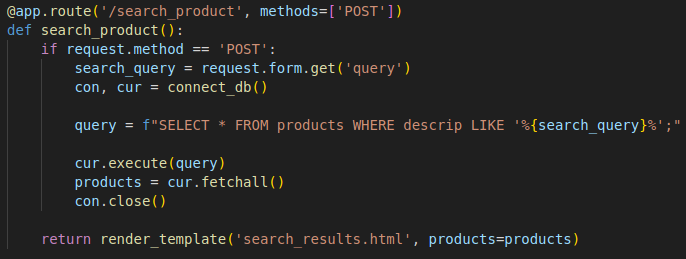
\includegraphics[width=16cm]{images/CWE-20_cod1v.png}
      \caption{CWE-20: Versão Insegura: @app.route search\_product() - Base de Dados(app.py)}
      \label{fig:cwe20-cod1v}
    \end{figure}
%%
\subsubsection{Correcção (app\_sec):}
Para corrigir esta vulnerabilidade e evitar futuras ocorrências da mesma, migrámos do uso de SQLite, que não oferece proteções robustas contra injeção de SQL, para SQLAlchemy. \\

Esta abordagem é mais segura, SQLAlchemy lida garante a separação segura dos dados do utilizador e do código SQL em queries, protegendo a aplicação contra a injeção de SQL e outras vulnerabilidades relacionadas à entrada de dados. \\

Foi usada a bibioteca \textit{"bleach"}, que sanitiza os inputs dos utilizadores e foi efectuada a parametrização das \textit{queries} recorrendo à função \textit{"text"} de SQLAlchemy, prevenindo com maior eficácia assim ataques \textbf{XSS} ou \textbf{SQL Injection}, tal como demonstrado na Figura \ref{fig:cwe20-cod1s}.\\

\begin{figure}[H]
  \centering
  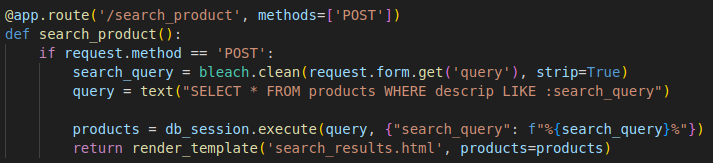
\includegraphics[width=16cm]{images/CWE-20-cod1s.png}
  \caption{CWE-20: Versão Segura: @app.route search\_product() - Base de Dados(app\_sec.py)}
  \label{fig:cwe20-cod1s}
\end{figure}
%
%
%%%%%%%%%%%%%%%%%%%%%%%%%%%%%%%%%%%%%%%%%%%
\section{CWE-79: Improper Neutralization of Input During Web Page Generation ('Cross-site Scripting')}
\label{sec.cwe79}

Conhecida por \textit{"Cross-site Scripting"} ou \textit{XSS}), esta vulnerabilidade ocorre quando uma aplicação não consegue neutralizar adequadamente os inputs efectuados deliberadamente pelo utilizador antes de os usar como output, sendo efectuado o display deste output a outros utilizadores, compromentendo assim a integridade e segurança da solução web, permitindo aos atacantes injetar código malicioso, como JavaScript, nos navegadores de outros utilizadores. \\
Como tal é importante seguir boas práticas de segurança e programação no desenvolvimento de aplicações web, minimizando o risco de uma exploração \textit{"Cross-site Scripting"}, por forma a proteger os utilizadores finais contra potenciais ameaças. \\
Existem três tipos principais de XSS:

    \begin{itemize}
        \item \textbf{Reflected \textit{XSS} (Não Persistente):} O servidor lê diretamente os dados a partir do pedido HTTP e reflete-os na sua resposta HTTP. Ocorre quando um atacante "força" (indirectamente) uma vítima a fornecer conteúdo perigoso a uma aplicação web vulnerável, que é posteriormente refletido de volta para a vítima e executado pelo navegador web. O mecanismo mais comum para a entrega de conteúdo malicioso é incluí-lo como um parâmetro numa URL que é publicada ou enviada diretamente à vítima, sendo que não é armazenada em Base de Dados (não persistente). 
        \item \textbf{Stored \textit{XSS} (Persistente):} Um atacante armazena dados perigosos na base de dados usando mensagens em forums, comentários, ou outras áreas exibida a muitos utilizadores. Posteriormente, os dados perigosos são "lidos" pela aplicação e incluídos em conteúdo dinâmico que, ao ser executado por um utilizador, permite ao atacante realizar operações privilegiadas em nome do utilizador (ou aceder a dados sensíveis deste).
        \item \textbf{DOM-Based \textit{XSS}:} Neste caso é o utilizador que realiza a injeção de XSS na página web \textit{(client sided)}. Geralmente envolve script confiável controlado pelo servidor que é enviado para o cliente. Se o script fornecido pelo servidor processar dados fornecidos pelo utilizador e depois os injetar de volta na página web, então o DOM-Based XSS é possível.
    \end{itemize}
    
\subsubsection{Demonstração e Impacto (app)}

Esta vulnerabilidade está presente nas funções, \textbf{login()}, \textbf{rate\_comment\_product\_route()}, \textbf{add\_product()}, \textbf{search\_product()}, entre outras.
Todas estas funções estão suscetíveis a Cross-Site-Scripting, devido à falta de validação de dados inseridos pelo utilizador, levando à possibilidade de inserção de scripts maliciosos.
A função \textbf{rate\_comment\_product\_route()}, como podemos observar pelas Figuras \ref{fig:cwe79-rateProduct}, \ref{fig:cwe79-JS1}, \ref{fig:cwe79-JS3} e \ref{fig:cwe79-JS2} são um excelente exemplo de como esta vulnerabilidade poderia afetar o website, visto que permite exibição de conteúdos indesejados para todos os utilizadores.

\begin{figure}[H]
  \centering
  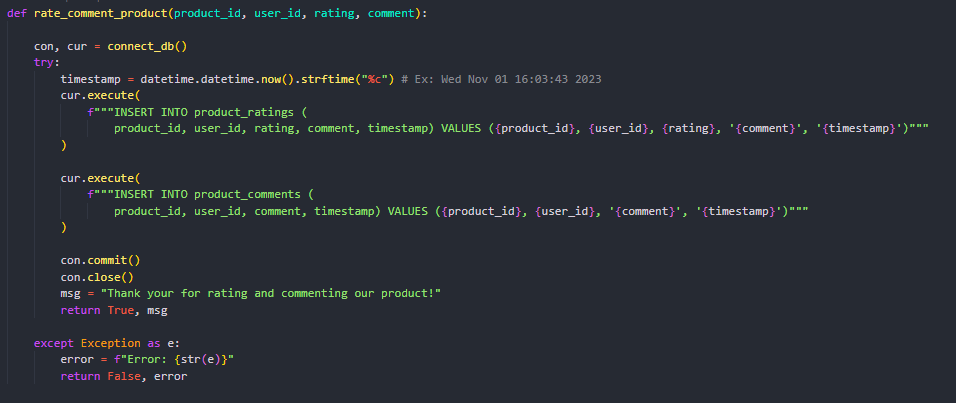
\includegraphics[width=16cm]{images/CWE79-rateProduct.png}
  \caption{CWE-79: Versão Insegura: @app.route rate\_comment\_product\_route() - Base de Dados(app.py)}
  \label{fig:cwe79-rateProduct}
\end{figure}

\begin{figure}[H]
  \centering
  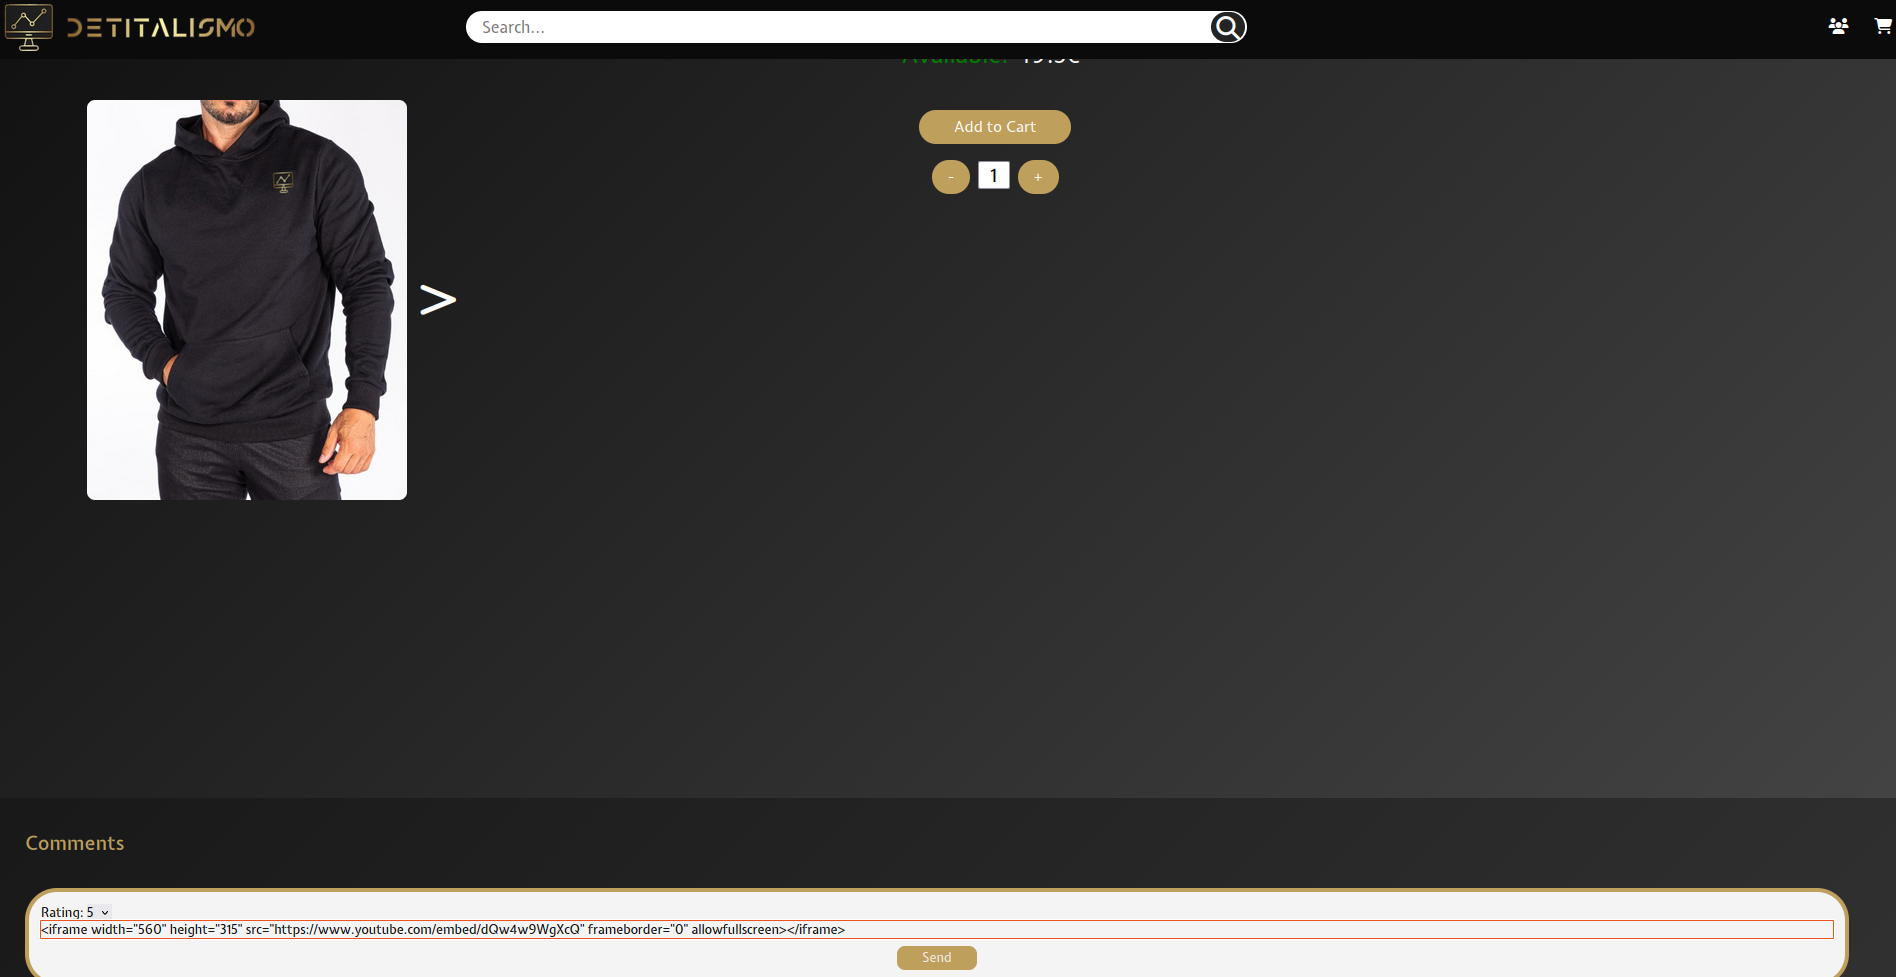
\includegraphics[width=16cm]{images/CWE-79-1.png}
  \caption{CWE-79: Versão Insegura: Comentário JS em Front-end (Product: Hoodie)}
  \label{fig:cwe79-JS1}
\end{figure}

\begin{figure}[H]
  \centering
  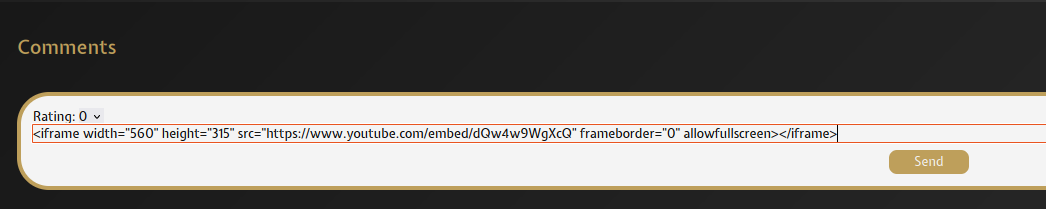
\includegraphics[width=16cm]{images/CWE-79-3.png}
  \caption{CWE-79: Versão Insegura: Comentário JS em Front-end (Product: Hoodie)}
  \label{fig:cwe79-JS3}
\end{figure}

\begin{figure}[H]
  \centering
  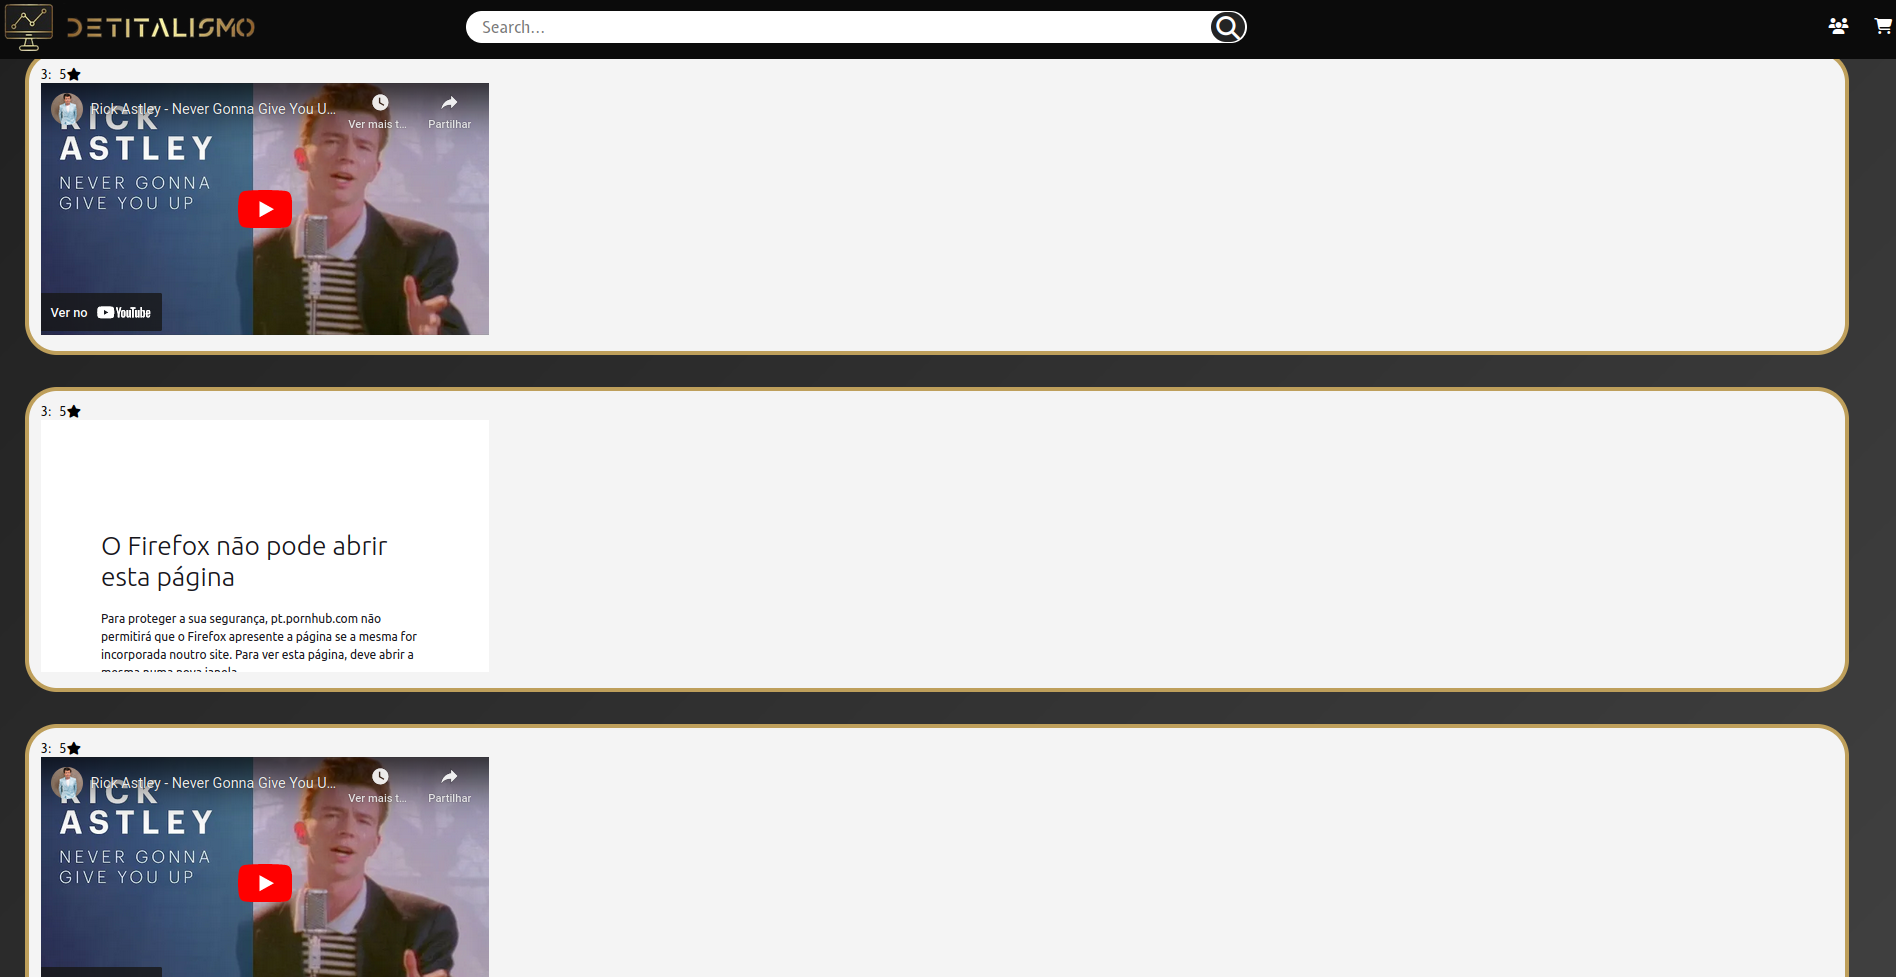
\includegraphics[width=16cm]{images/CWE-79-2.png}
  \caption{CWE-79: Versão Inesgura: Resultado XSS Attack Front-end (Product: Hoodie)}
  \label{fig:cwe79-JS1}
\end{figure}

\subsubsection{Correcção (app\_sec):}

Para corrigir esta vulnerabilidade, foi usada a bibioteca de \textbf{Python} \textit{"bleach"}, que sanitiza os inputs dos utilizadores e foi efectuada a parametrização das \textit{queries} recorrendo à função \textit{"text"} de SQLAlchemy, prevenindo com maior eficácia ataques de \textbf{XSS}, tal como demonstrado na Figura \ref{fig:cwe79-rateProduct-Secure}.\\

\begin{figure}[H]
  \centering
  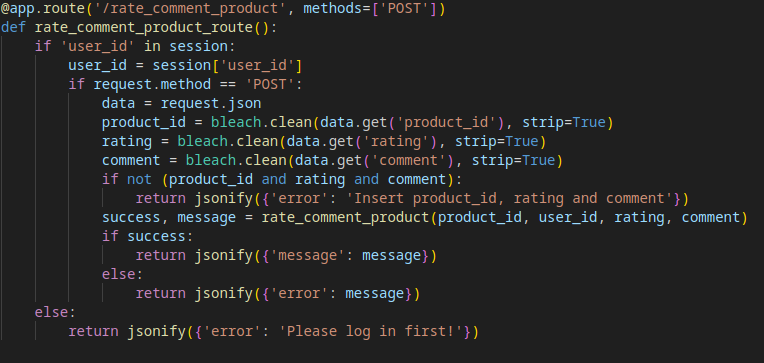
\includegraphics[width=16cm]{images/CWE79-rateProduct-Secure.png}
  \caption{CWE-79: Versão Segura: @app.route rate\_comment\_product\_route() - Base de Dados(app\_sec.py)}
  \label{fig:cwe79-rateProduct-Secure}
\end{figure}


%
%
%%%%%%%%%%%%%%%%%%%%%%%%%%%%%%%%%%%%%%%%%%%
\section{CWE-89: Improper Neutralization of Special Elements used in an SQL Command ('SQL Injection')}
\label{sec.cwe89}
Também conhecida por \textit{"SQL Injection"}, esta vulnerabilidade ocorre quando se pede a um usuário que forneça um input, como o username, e em vez do username é inserida uma declaração SQL que irá atacar a base de dados. 
Esta vulnerabilidade permite que o utilizador leia, modifique e elimine dados sensíveis, comprometendo assim a integridade dos mesmos. 
No contexto do nosso projeto, a aplicação insegura é vulnerável a injeções de SQL, pois não foi realizada a devida prévia validação e saneamento dos dados introduzidos pelos utilizadores. 

\subsubsection{Demonstração e Impacto (app)}

Aplicada ao projeto em questão, podemos verificar que esta vulnerabilidade encontra-se presente no código, na maioria das funções e rotas da base de dados da app vulnerável. Esta occorre quando o input do utilizador é utilizado diretamente numa declaração SQL.
As rotas nas quais esta vulnerabilidade pode ser encontrada são: 

\begin{itemize}
    \item \textbf{register()}
    \item \textbf{login()}
    \item \textbf{change\_password()}
    \item \textbf{mecart()}
    \item \textbf{upCart()}
    \item \textbf{rate\_comment\_product\_route()}
    \item \textbf{search\_product()}
    \item \textbf{get\_items()}
    \item \textbf{add\_product\_route()}
\end{itemize}


\begin{figure}[H]
  \centering
  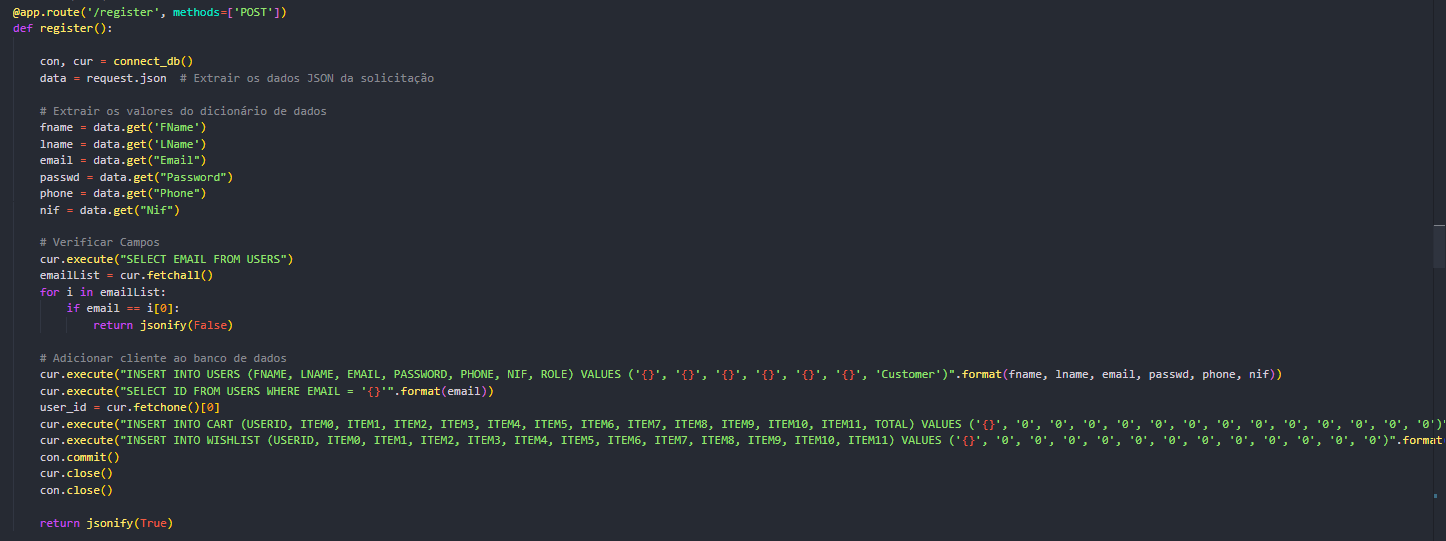
\includegraphics[width=16cm]{images/CWE-89-Register.png}
  \caption{CWE-89: Versão Insegura: @app.route register() - Base de Dados(app.py)}
  \label{fig:cwe89-register}
\end{figure}

\begin{figure}[H]
  \centering
  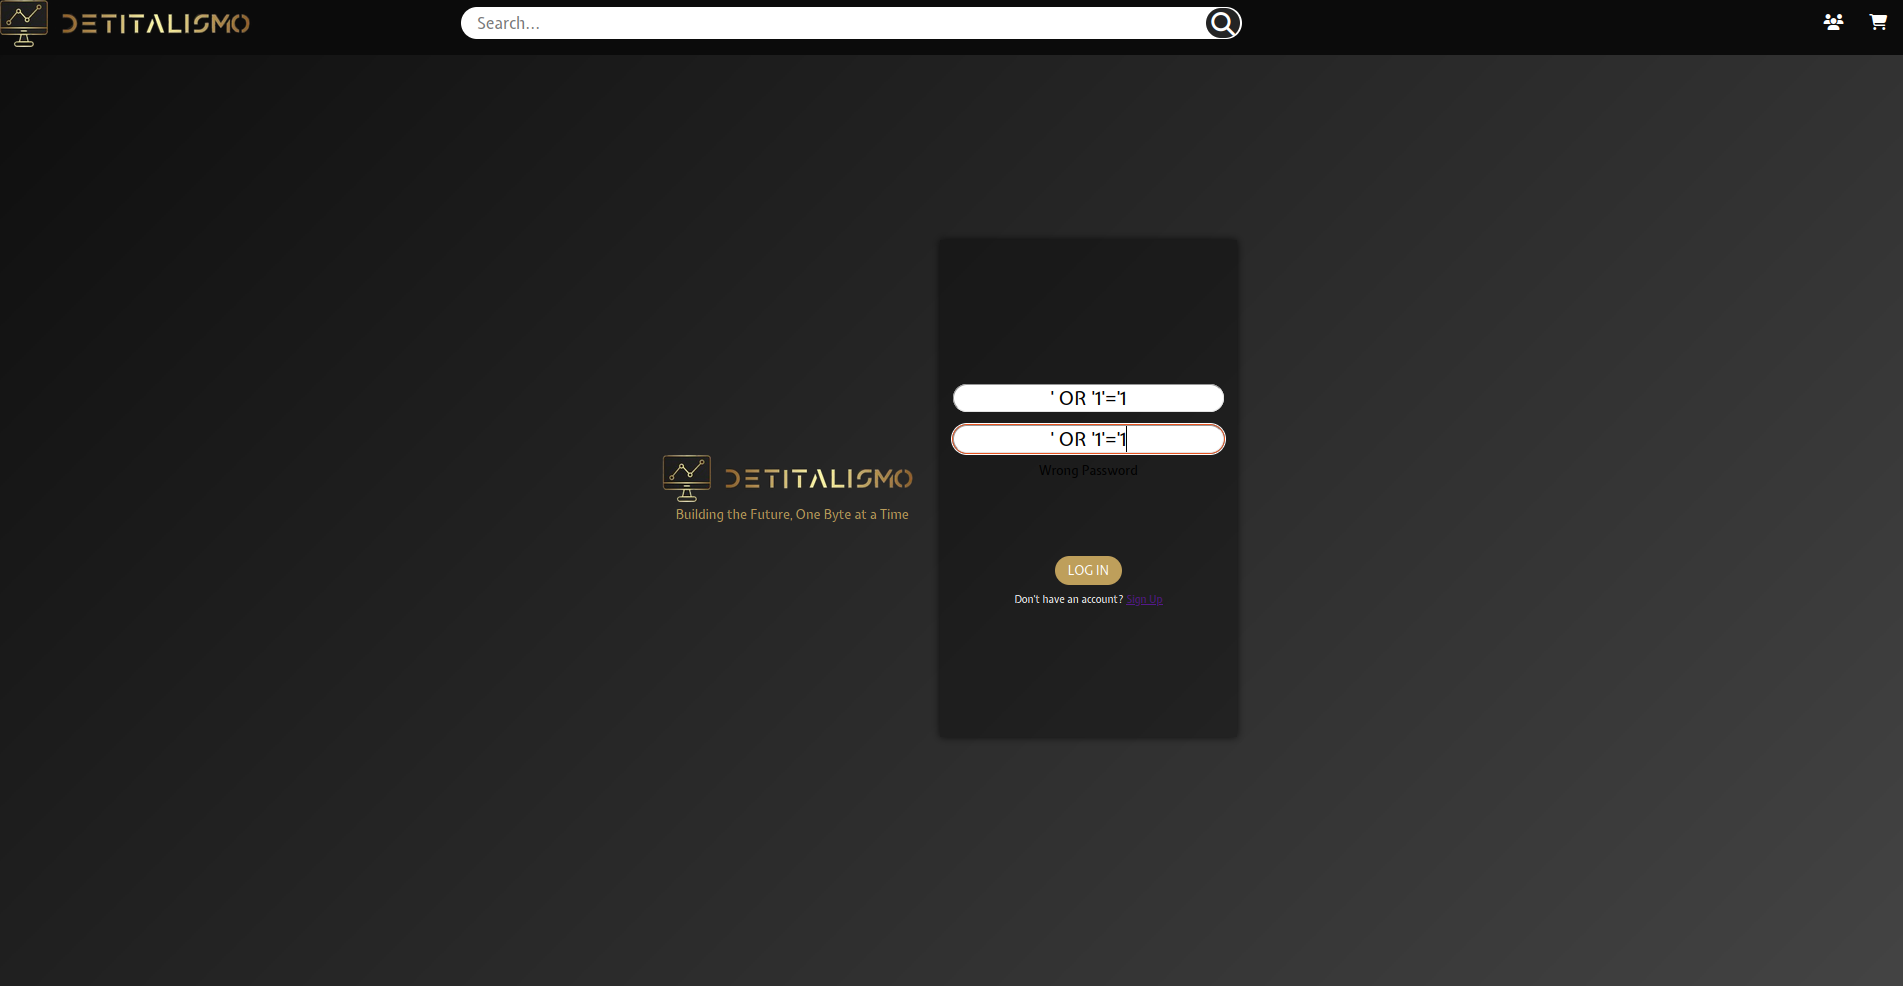
\includegraphics[width=16cm]{images/CWE-89-Inject.png}
  \caption{CWE-89: Versão Insegura: User Interface Front-End: Tentativa SQL Injection}
  \label{fig:cwe89-inject}
\end{figure}

\begin{figure}[H]
  \centering
  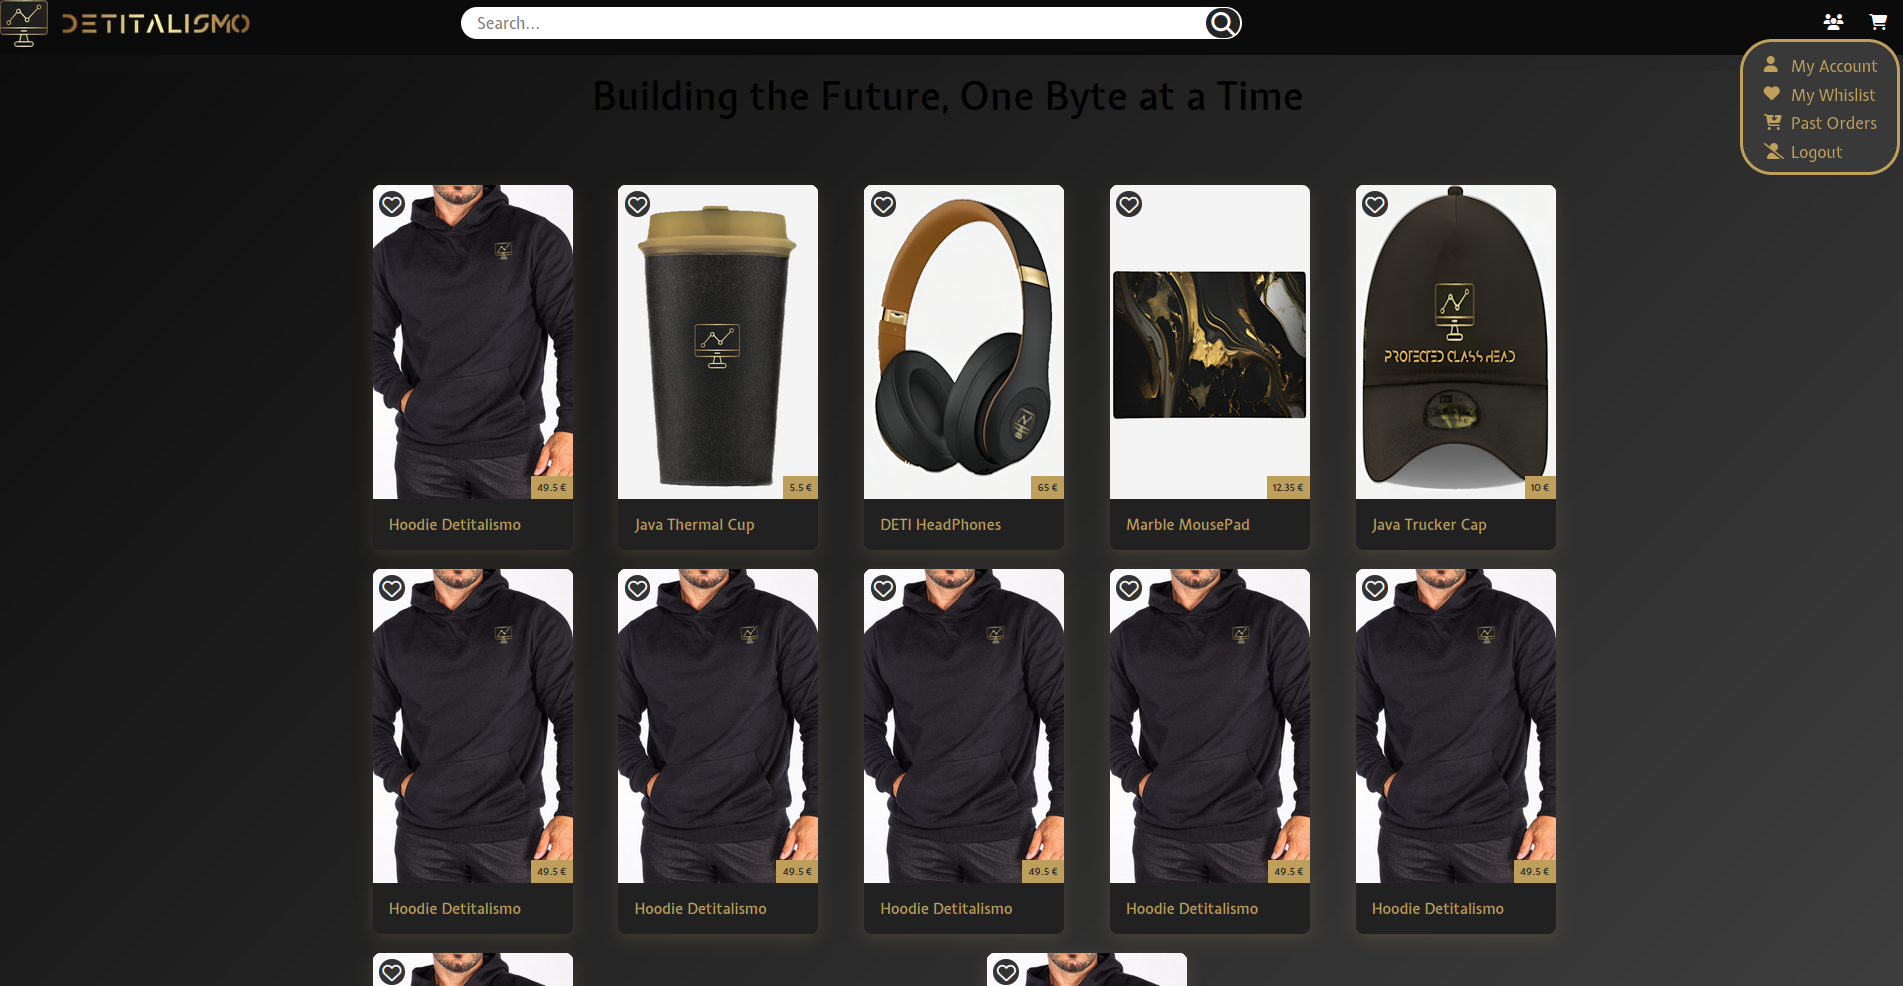
\includegraphics[width=16cm]{images/CWE-89-Sucess.png}
  \caption{CWE-89: Versão Insegura: User Interface Front-End: Sucesso de SQL Injection}
  \label{fig:cwe89-sucess}
\end{figure}

Como podemos observar pelas Figuras \ref{fig:cwe89-register} e \ref{fig:cwe89-inject}, não existe qualquer tipo de validação e saneamento dos dados introduzidos pelo utilizador, sendo estes utilizados numa declaração SQL.

\subsubsection{Correcção (app\_sec):}

Para corrigir esta vulnerabilidade, foi usada a bibioteca de \textbf{Python} \textit{"bleach"}, que sanitiza os inputs dos utilizadores e foi efectuada a parametrização das \textit{queries} recorrendo à função \textit{"text"} de SQLAlchemy, prevenindo com maior eficácia assim ataques ou \textbf{SQL Injection}, tal como demonstrado na Figura \ref{fig:cwe89-register-secure}.\\


\begin{figure}[H]
  \centering
  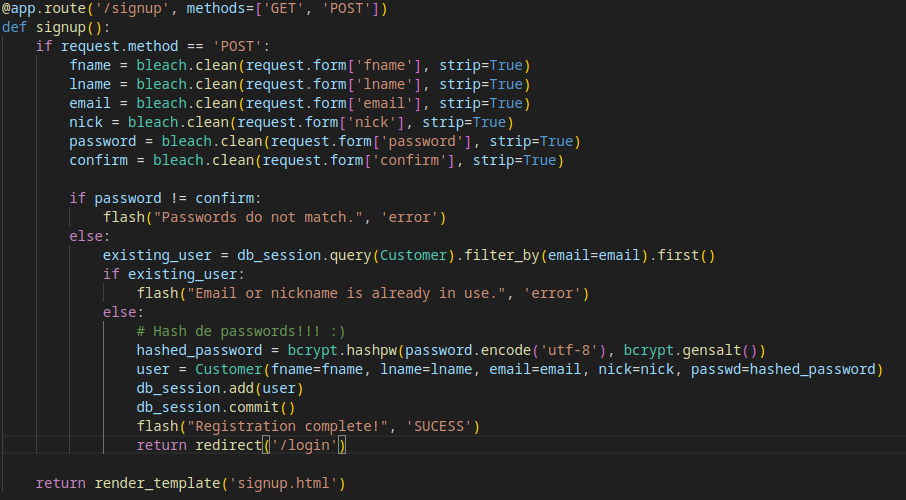
\includegraphics[width=16cm]{images/CWE89-Register-Secure.png}
  \caption{CWE-89: Versão Segura: @app.route register() - Base de Dados(app\_sec.py)}
  \label{fig:cwe89-register-secure}
\end{figure}

%
%
%%%%%%%%%%%%%%%%%%%%%%%%%%%%%%%%%%%%%%%%%%%
\section{CWE-200: Exposure of Sensitive Information to an Unauthorized Actor}
\label{sec.cwe200}

A exposição de informações sensíveis a atores não autorizados é uma vulnerabilidade grave que pode ocorrer quando dados confidenciais são acessíveis por indivíduos não autorizados. Pode resultar em:

\begin{itemize}
    \item Violações de privacidade 
    \item Roubo de identidade
    \item Perda de propriedade intelectual
    \item Outros impactos prejudiciais
\end{itemize}


Neste projecto, torna-se especialmente relevante ao no front-end da aplicação, onde dá \textit{feedback} aos utilizadores sobre que campo (email ou password) se encontra incorreto durante uma tentativa de login incorrecta, revelando mais informações do que seria necessário, permitindo que um possível atacante explore com mais facilidade uma entrada não autorizada por tentativa/erro. 

\subsubsection{Demonstração e Impacto (app)}

\begin{figure}[H]
  \centering
  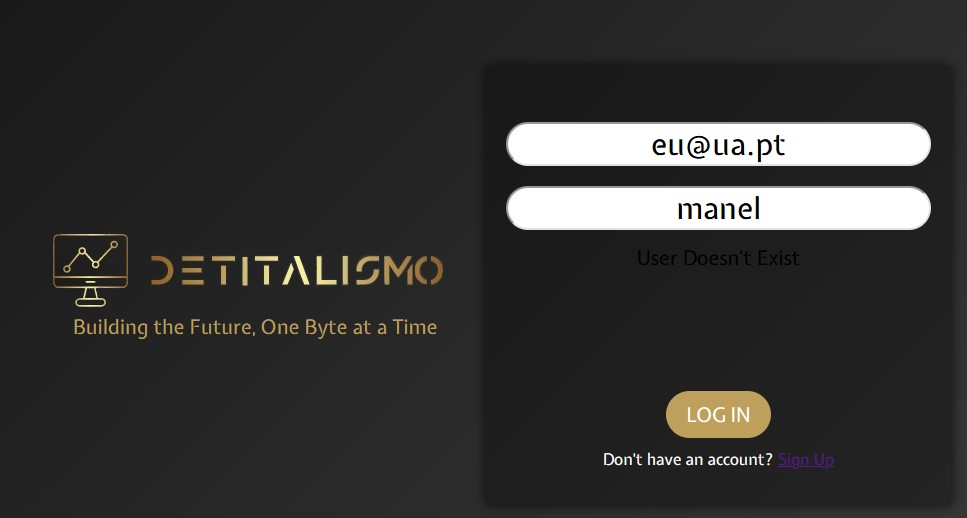
\includegraphics[width=16cm]{images/CWE-200-vulneravel1.jpg}
  \caption{CWE-200: Versão Insegura: "User doesn't exist" : User Interface Front-end Login }
  \label{fig:cwe200-vulneravel1}
\end{figure}

\begin{figure}[H]
  \centering
  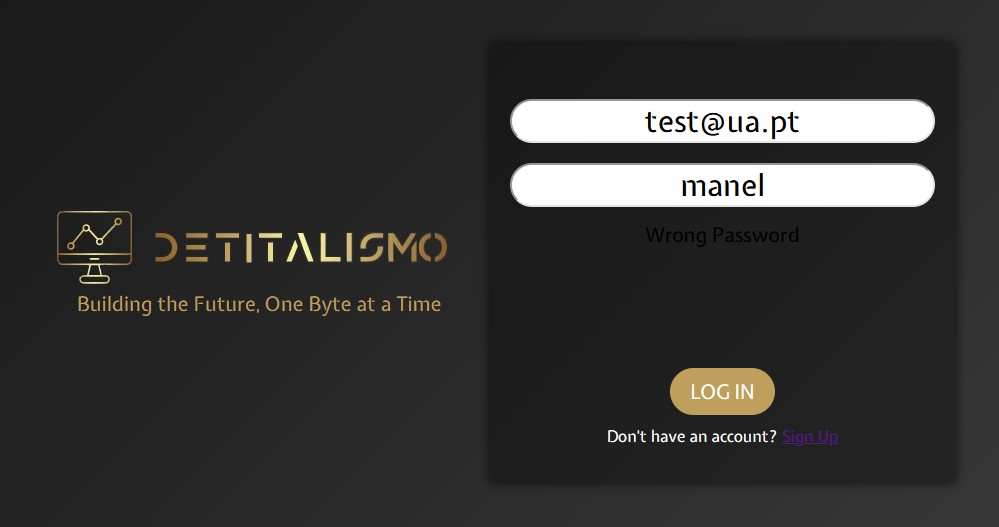
\includegraphics[width=16cm]{images/CWE-200-vulneravel2.jpg}
  \caption{CWE-200: Versão Insegura: "Wrong Password": User Interface Front-end Login }
  \label{fig:cwe200-vulneravel2}
\end{figure}

\begin{figure}[H]
  \centering
  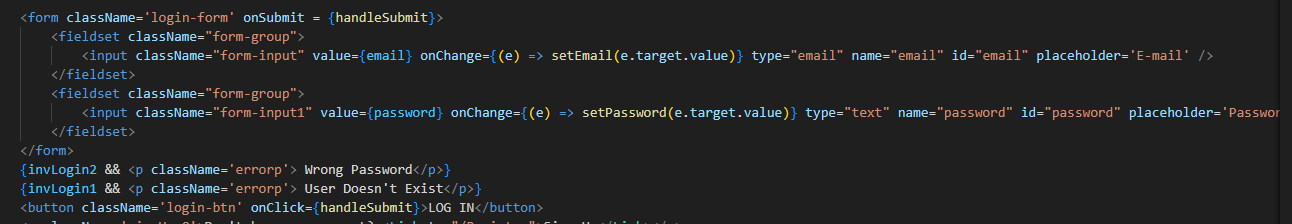
\includegraphics[width=16cm]{images/CWE-200-cod1v.png}
  \caption{CWE-200: Versão Insegura: Código inseguro Front-end Login }
  \label{fig:cwe200-cod1v}
\end{figure}

\subsubsection{Correcção (app\_sec):}

\begin{figure}[H]
  \centering
  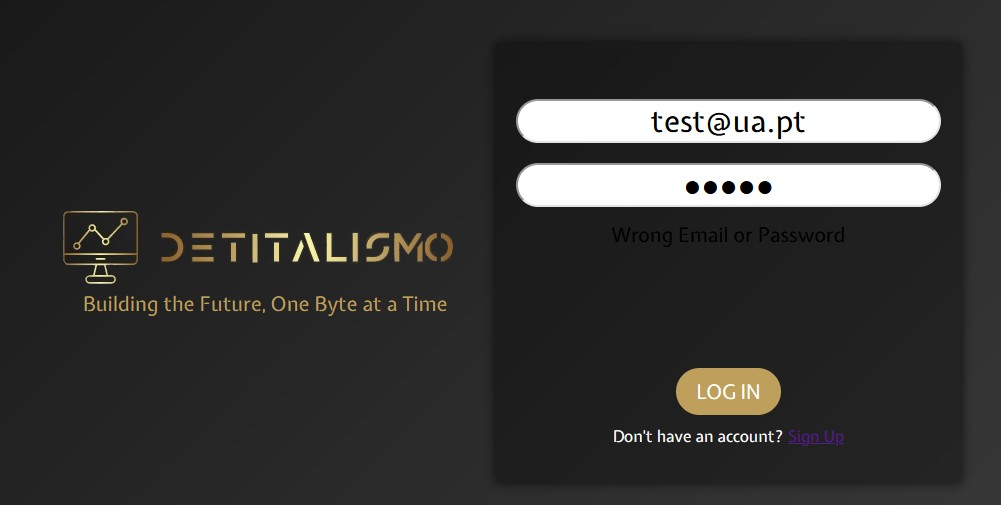
\includegraphics[width=16cm]{images/CWE-200-segura.jpg}
  \caption{CWE-200: Versão Segura corrigida: Front-end Login }
  \label{fig:cwe200-segura}
\end{figure}

\begin{figure}[H]
  \centering
  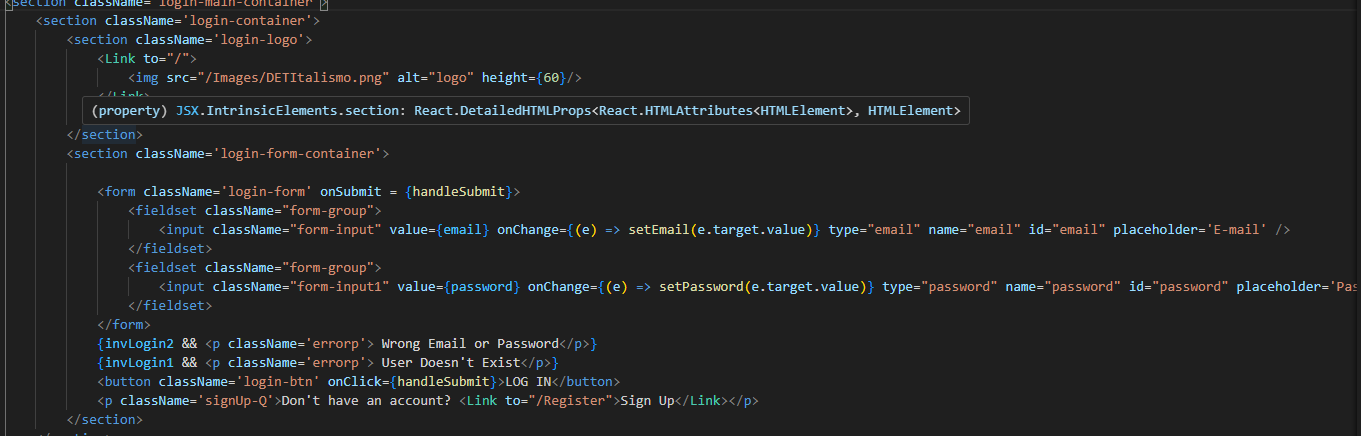
\includegraphics[width=16cm]{images/CWE-200-cod1s.png}
  \caption{CWE-200: Versão Segura: Código Corrigido Front-end Login }
  \label{fig:cwe200-cod1s}
\end{figure}

%
%
%%%%%%%%%%%%%%%%%%%%%%%%%%%%%%%%%%%%%%%%%%%
\section{CWE-256: Plaintext Storage of a Password}
\label{sec.cwe256}
A vulnerabilidade CWE-256, é uma vulnerabilidade comum que se refere aos problemas que ocorrem quando password são armazenadas em texto simples nas propriedades da aplicação, nos ficheiros de configuração ou na memória. Esta torna as password acessíveis a qualquer entidade com acesso aos ficheiros onde estas estão guardadas. A mitigação desta vulnerabilidade requer a utilização de algoritmos de hash criptográfico sobre as password e armazenamento do hash resultante.
\\
\subsubsection{Demonstração e Impacto (app)}
No projecto, esta vulnerabilidade é evidente através da análise do código responsável pela construção das tabelas de utilizadores e sua inserção (Nota: utilizadores são chamados de \textit{customers}) e da visualização da base de dados em questão, tal como demonstrado nas Figuras \ref{fig:cwe256-cod1s} e \ref{fig:cwe256-BDv} seguintes:

\begin{figure}[H]
  \centering
  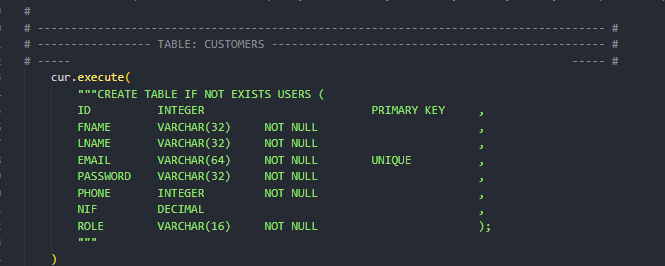
\includegraphics[width=16cm]{images/CWE-256-cod1v.png}
  \caption{CWE-256: Versão Insegura: Tabela e Inserts de "Customers" - Base de Dados(app.py)}
  \label{fig:cwe256-cod1s}
\end{figure}

\begin{figure}[H]
  \centering
  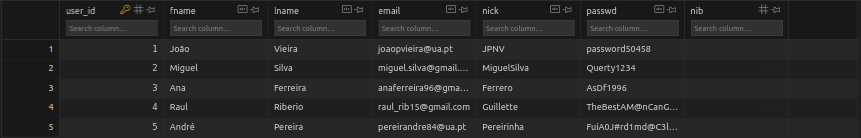
\includegraphics[width=16cm]{images/CWE-256-BDv.png}
  \caption{CWE-256: Versão Insegura: Interior da Base de Dados criada (DOSG26.db)}
  \label{fig:cwe256-BDv}
\end{figure}

Como se pode verificar, as \textit{passwords} dos utilizadores inseridos são guardadas (de forma incorrecta/vulnerável) em texto (plaintext), tal como dita a vulnerabilidade.

\subsubsection{Correcção (app\_sec):}
Para corrigir este problema, foram executadas as seguintes alterações demonstradas nas Figuras \ref{fig:cwe256-hash} e \ref{fig:cwe256-BDs}:

\begin{figure}[H]
  \centering
  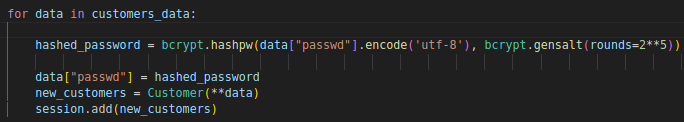
\includegraphics[width=16cm]{images/CWE-256-Hashing.png}
  \caption{CWE-256: Versão Segura: Hashing de Passwords antes de "insert" - Base de Dados(db\_inserts.py)}
  \label{fig:cwe256-hash}
\end{figure}

\begin{figure}[H]
  \centering
  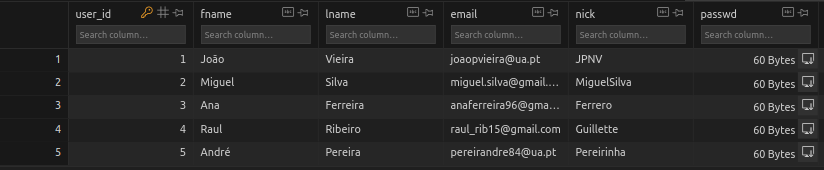
\includegraphics[width=16cm]{images/CWE-256-BDs.png}
  \caption{CWE-256: Versão Segura: Interior da Base de Dados criada (DOSG26\_SEC.db)}
  \label{fig:cwe256-BDs}
\end{figure}

Como se pode verificar, recorrendo à função hash criptográfica \textit{"bcrypt"} e metodos de \textit{"salting"} (com $2^5$ iterações/rounds, para maior segurança), para corrigir o problema. 

%
%
%%%%%%%%%%%%%%%%%%%%%%%%%%%%%%%%%%%%%%%%%%%
\section{CWE-284: Improper Access Control}
\label{sec.cwe284}

A vulnerabilidade CWE-284, refere-se ao acesso inadequado. Ocorre quando não é feito o devido controlo ao acesso de recursos sensíveis. Pode levar a acessos não autorizados, representando uma ameaça significativa para a integridade dos sistemas e dos seus dados.
Para mitigar esta vulnerabilidade, é fundamental implementar uma política de controle de acesso bem definida, que inclua uma forte autenticação.

\subsubsection{Demonstração e Impacto (app)}

No contexto do nosso projeto, podemos verificar que esta vulnerabilidade encontra-se presente no código. Apesar de na base de dados se poder armazenar Admins e Customers, existem funções que deviam ser restritas apenas a admins, no entanto não existe qualquer verificação para o tipo de utilizador (Customer ou Admin) que está a fazer o request. 

\begin{figure}[H]
  \centering
  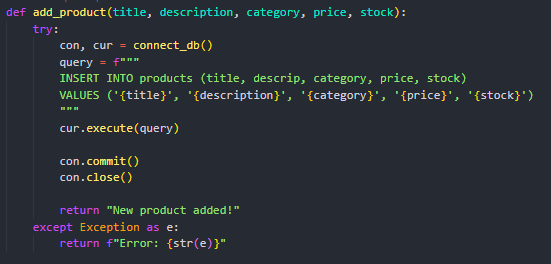
\includegraphics[width=16cm]{images/CWE-284-product_route.png}
  \caption{CWE-284: Versão Insegura: @app.route add\_product\_route() - Base de Dados(app.py)}
  \label{fig:cwe284-add-product-route}
\end{figure}

\begin{figure}[H]
  \centering
  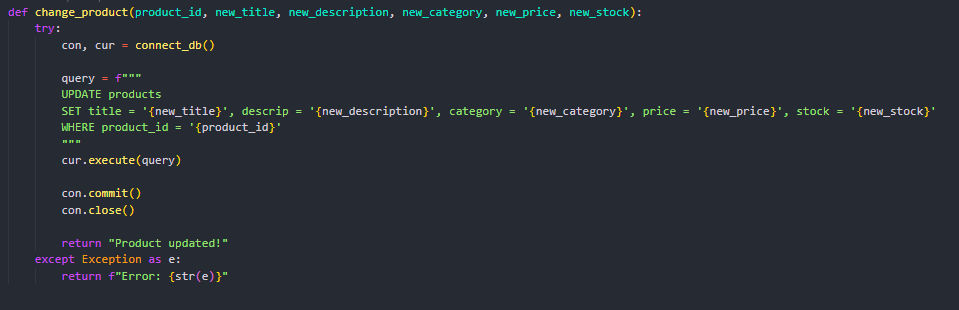
\includegraphics[width=16cm]{images/CWE-284-change_product_route.png}
  \caption{CWE-284: Versão Insegura: @app.route change\_product\_route() - Base de Dados(app.py)}
  \label{fig:cwe284-change-product-route}
\end{figure}

Como podemos observar pela Figura \ref{fig:cwe284-add-product-route} e \ref{fig:cwe284-change-product-route}, qualquer utilizador, Customer ou Admin consegue adicionar e alterar os produtos do nosso website.
 

\subsubsection{Correcção (app\_sec):}

Esta vulnerabilidade foi corrigida através da verificação do campo "Role", presente em todos os utilizadores. Assim existem funções restritas apenas aos Admins.


\begin{figure}[H]
  \centering
  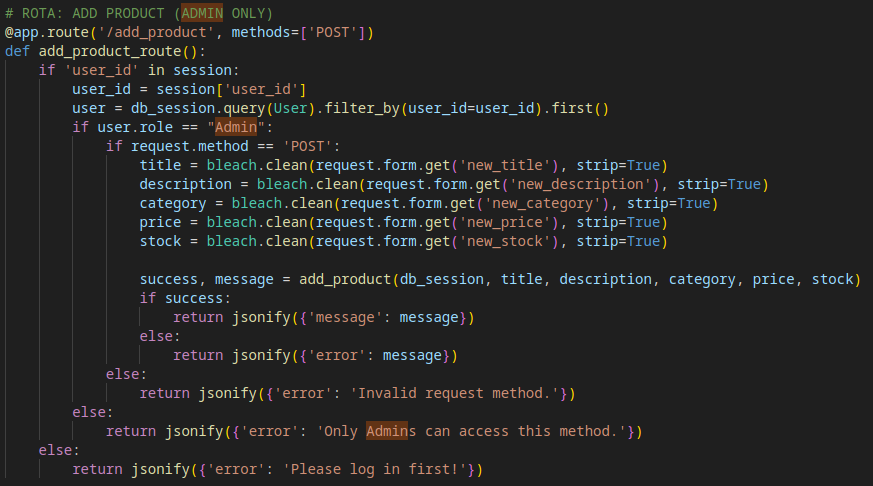
\includegraphics[width=16cm]{images/CWE-284-product_route-secure.png}
  \caption{CWE-284: Versão Segura: @app.route add\_product\_route() - Base de Dados(app\_sec.py)}
  \label{fig:cwe284-add-product-route-secure}
\end{figure}

\begin{figure}[H]
  \centering
  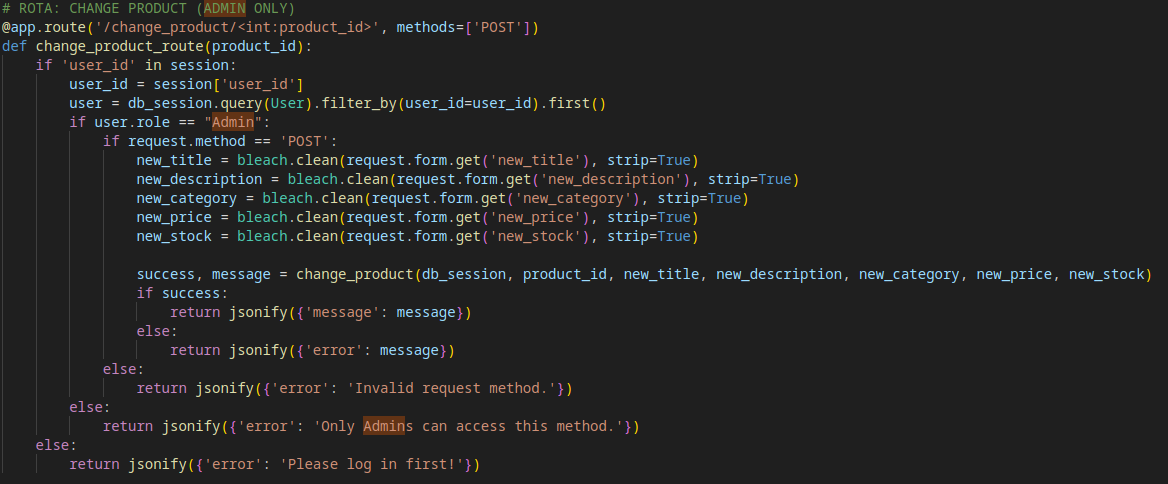
\includegraphics[width=16cm]{images/CWE-284-change_product_route-secure.png}
  \caption{CWE-284: Versão Segura: @app.route change\_product\_route() - Base de Dados(app\_sec.py)}
  \label{fig:cwe284-change-product-route-secure}
\end{figure}

%
%
%%%%%%%%%%%%%%%%%%%%%%%%%%%%%%%%%%%%%%%%%%%
\section{CWE-307: Improper Restriction of Excessive Authentication Attempts}
\label{sec.cwe307}
A aplicação web não implementa medidas suficientes para evitar múltiplas tentativas de autenticação por um atacante num curto espaço de tempo, tornanda assim mais suscetível a ataques de força bruta, onde um atacante tenta incessantemente adivinhar passwords ou outras formas de credenciais de acesso.

\subsubsection{Demonstração e Impacto (app)}

\begin{figure}[H]
  \centering
  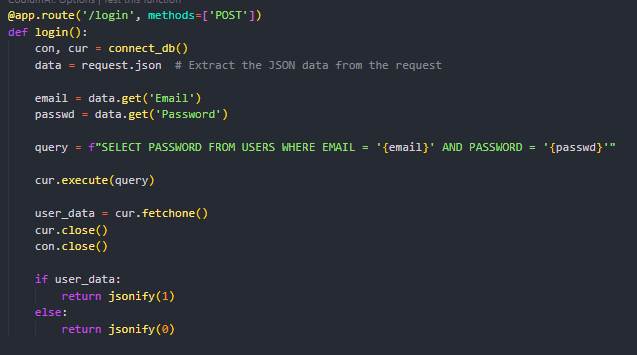
\includegraphics[width=0.8\linewidth]{images/CWE307-unsafe-app.png}
  \caption{CWE-307: Versão Insegura: @app.route login() - Base de Dados(app\_sec)}
  \label{fig:cwe307-unsafe-app}
\end{figure}

\subsubsection{Correcção (app\_sec):}
Primeiramente foi decidido implementar um contador de tentativas de login. Fazendo com que quando atingisse 5 tentativas falhadas seguidas, a conta fosse bloqueada e para recuperar seria necessário o contactar o suporte. Para tal foi adicionada à tabela da base de dados a failed\_login\_attemps ,figura \ref{fig:cwe307-safe-sec_db_tables}, para o seu valor poder ser incrementado, figura \ref{fig:cwe307-safe-sec_app}.
\begin{figure}[H]
  \centering
  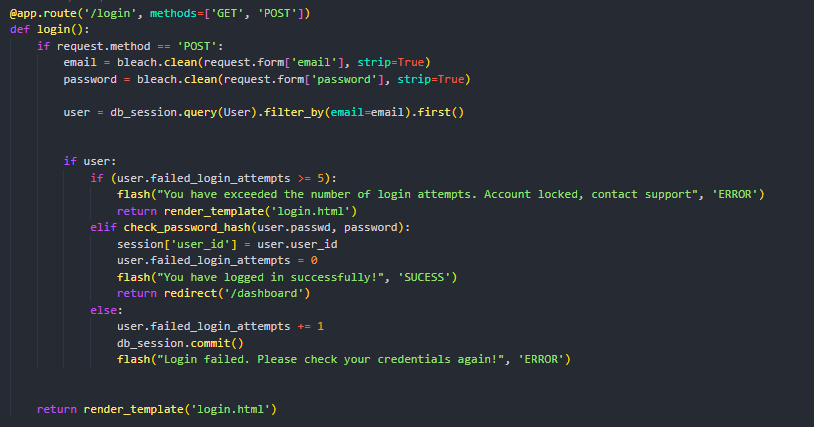
\includegraphics[width=0.8\linewidth]{images/CWE307-safe-sec_app.png}
  \caption{CWE-307: Versão Insegura: @app.route login() - Base de Dados(app\_sec.py)}
  \label{fig:cwe307-safe-sec_app}
\end{figure}
\begin{figure}[H]
  \centering
  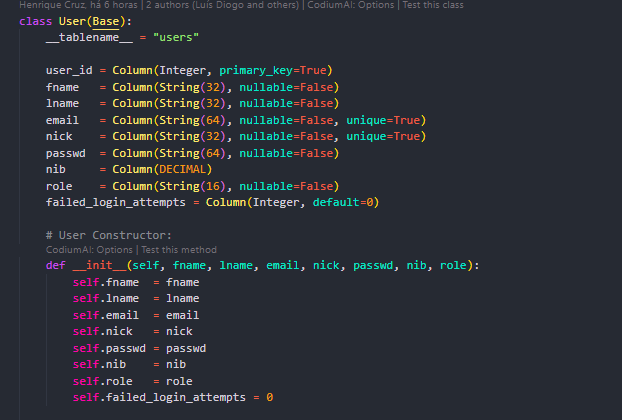
\includegraphics[width=0.8\linewidth]{images/CWE307-safe-sec_db_tables.png}
  \caption{CWE-307: Versão Insegura: - Base de Dados(db\_tables.py)}
  \label{fig:cwe307-safe-sec_db_tables}
\end{figure}
No fim foi concluído que esta implementação criaria uma vulnerabilidade onde qualquer conta seria facilmente bloqueada. Então decidimos optar por implementar uma taxa de tentativas de login limitadas ,como é possivel ver na figura \ref{fig:cwe307-safe2-sec_app} nas linhas 2 e 3, solucionando assim a vulnerabilidade.
\begin{figure}[H]
  \centering
  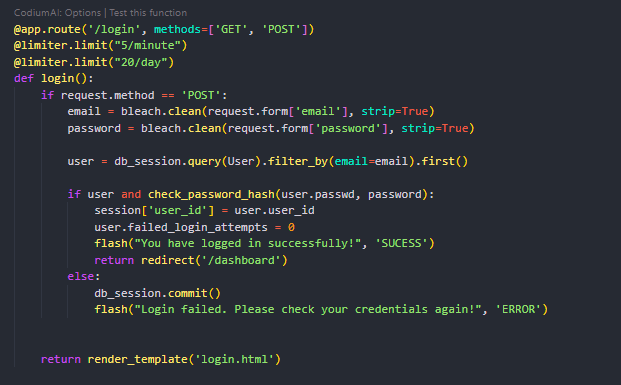
\includegraphics[width=0.8\linewidth]{images/CWE307-safe2-sec_app.png}
  \caption{CWE-307: Versão Segura: @app.route login() - Base de Dados(app\_sec.py)}
  \label{fig:cwe307-safe2-sec_app}
\end{figure}
%
%
%%%%%%%%%%%%%%%%%%%%%%%%%%%%%%%%%%%%%%%%%%%
\section{CWE-311: Missing Encryption of Sensitive Data}
\label{sec.cwe311}
Esta vulnerabilidade ocorre quando informações confidenciais, passwords, são armazenadas, transmitidas ou processadas sem a devida proteção criptográfica. \\
A falta de criptografia apropriada coloca em risco a confidencialidade e a integridade de dados, tornando-os vulneráveis a potenciais ameaças e violações de segurança. \\ 
Atacantes podem explorar essa vulnerabilidade para interceptar, aceder e/ou comprometer informações sensíveis, podendo resultar em roubo de identidade, fraude financeira, divulgação não autorizada de dados pessoais, etc...

\subsubsection{Demonstração e Impacto (app)}

No contexto do nosso projeto, podemos verificar que esta vulnerabilidade encontra-se presente no código.
O armazenamento das credencias dos utilizadores, bem como outros dados sensíveis são armazenados sem qualquer cifragem, diretamente na base de dados. 

\begin{figure}[H]
  \centering
  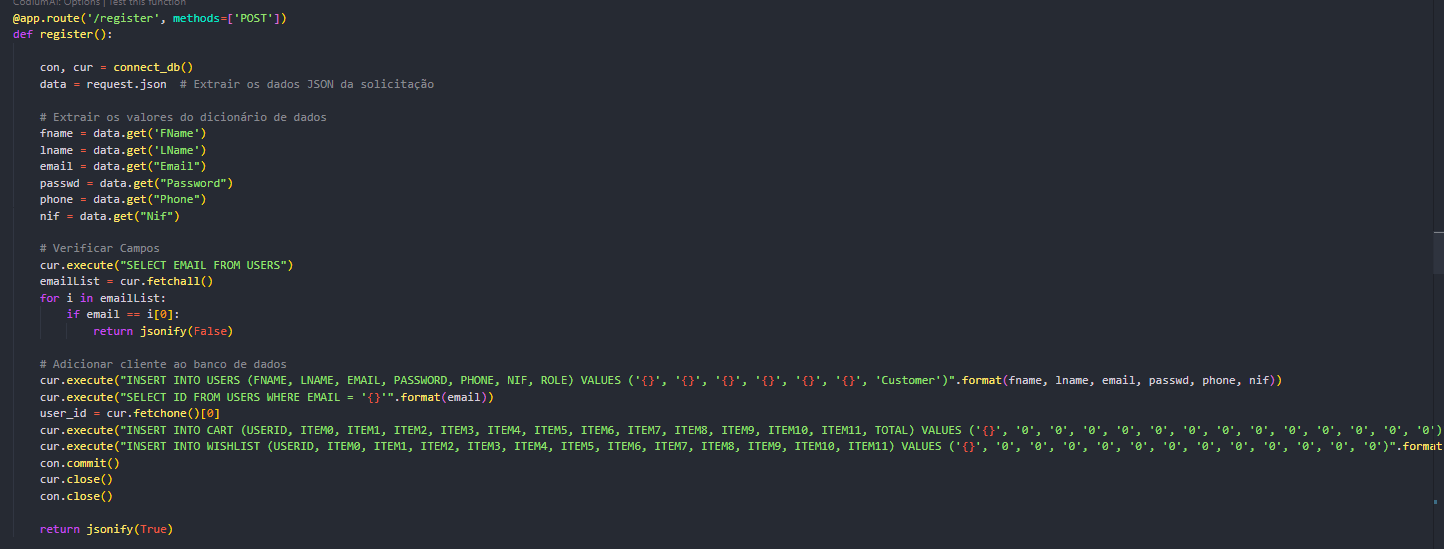
\includegraphics[width=16cm]{images/CWE-311-Register.png}
  \caption{CWE-311: Versão Insegura: @app.route register() - Base de Dados(app.py)}
  \label{fig:cwe311-register}
\end{figure}

No caso das credenciais dos admins, optámos por utilizar uma função hash com o algoritmo SHA-1, Figura  para realizar a cifragem, como podemos obervar pela Figura  \ref{fig:cwe311-hashFuntion}. Contudo esta é insegura porque não incorpora "salting" ou qualquer outro mecanismo de proteção adicional. O processo de "salting" é uma técnica fundamental que acrescenta uma \textit{string} aleatória e única à palavra-passe antes de aplicar a função de hash. Esta prática torna os hashes mais robustos, dificultando significativamente ataques de força bruta, por exemplo.

\begin{figure}[H]
  \centering
  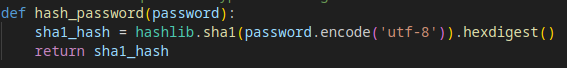
\includegraphics[width=16cm]{images/CWE-311-hashFunction.png}
  \caption{CWE-311: Versão Insegura: hash\_password() - Base de Dados(app.py)}
  \label{fig:cwe311-hashFuntion}
\end{figure}

\begin{figure}[H]
  \centering
  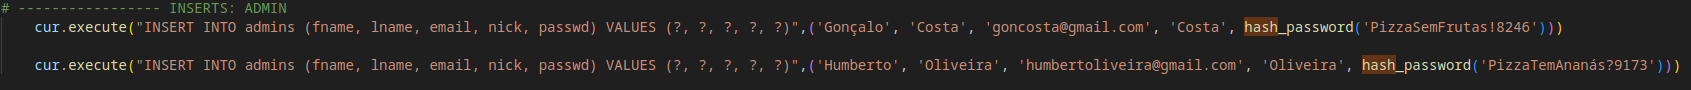
\includegraphics[width=16cm]{images/CWE-311-Admins.png}
  \caption{CWE-311: Versão Insegura: Inserir Credencias de Admins na Base de Dados - Base de Dados(app.py)}
  \label{fig:cwe311-admins}
\end{figure}


\subsubsection{Correcção (app\_sec):}

Para corrigir esta vulnerabilidade, foi usada a bibioteca de \textbf{Python} \textit{"bcrypt"}. Ao usar o \textit{"bcrypt"}, geramos um "salt" aleatório para cada palavra-passe antes de aplicar a função de hash. Este "salt" é então armazenado juntamente com o hash resultante. A inclusão do "salt" aumenta a complexidade do processo de hash, tornando-o mais difícil de ser descoberta.

\begin{figure}[H]
  \centering
  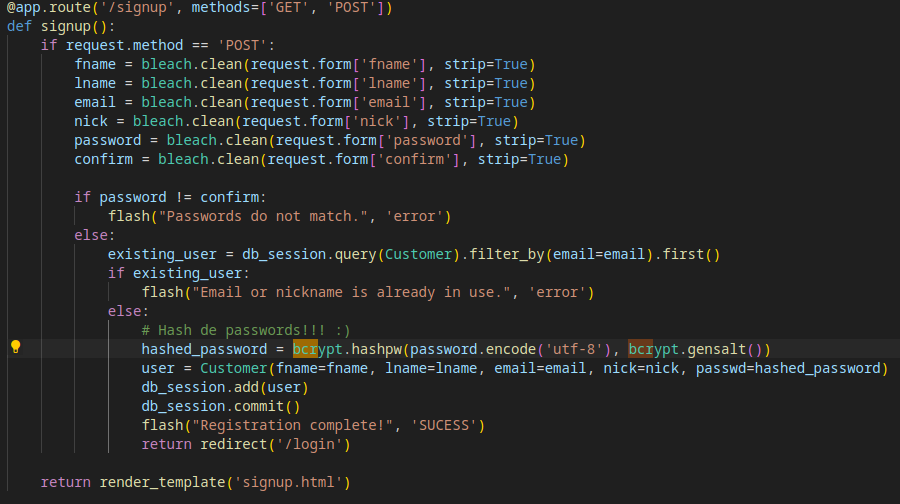
\includegraphics[width=16cm]{images/CWE-311-Register-Bcrypt.png}
  \caption{CWE-311: Versão Segura:  @app.route signup() - Base de Dados(app\_sec.py)}
  \label{fig:cwe311-register-bcrypt}
\end{figure}

%
%
%%%%%%%%%%%%%%%%%%%%%%%%%%%%%%%%%%%%%%%%%%%
\section{CWE-319: Cleartext Transmission of Sensitive Information}
\label{sec.cwe319}
Aplicações não devem transferir informações confidenciais ou sensíveis, sem a devida cifragem ou proteção. \\
No contexto da segurança de software, a CWE-319 realça os riscos associados ao envio de dados sensíveis em texto simples, tornando-os suscetíveis a escutas e interseções por parte de atacantes.

\subsubsection{Demonstração e Impacto (app)}
Para demonstração desta vulnerabilidade, pode-se analisar a rota de \textit{change\_password} apresentada na Figura seguinte:

\begin{figure}[H]
  \centering
  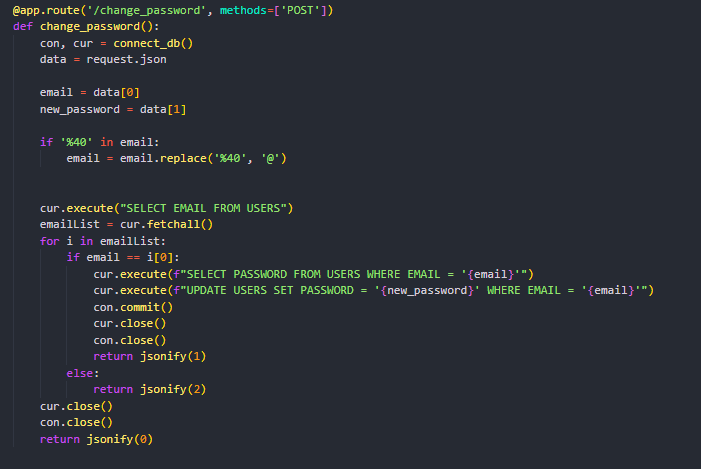
\includegraphics[width=16cm]{images/CWE-319-cod2v.png}
  \caption{CWE-319: Versão Insegura:  @app.route change\_password() - Base de Dados(app.py)}
  \label{fig:cwe319-cod2v}
\end{figure}

Nesta rota, é visível a clara falta de cifragem de informação sensível que passa por URLs e  um atacante com visibilidade de rede (por exemplo, Wireshark) pode interceptar esta informação.

\subsubsection{Correcção (app\_sec):}
Para corrigir foram aplicadas medidas de segurança como a biblioteca \textit{"bleach"} para "limpar" inputs de passwords, verificação de passwords e a hash function \textit{bcrypt} para proteger a password. 

\begin{figure}[H]
  \centering
  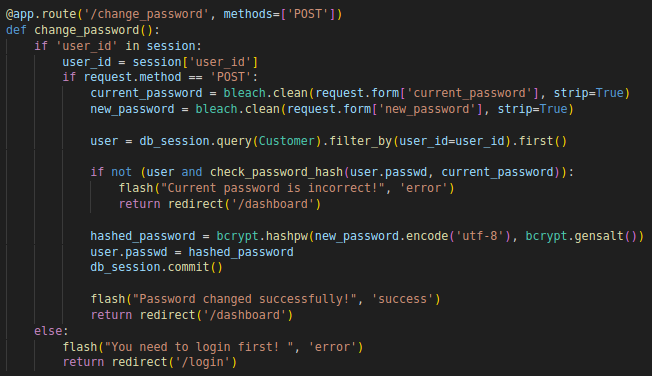
\includegraphics[width=16cm]{images/CWE-319-cod2s.png}
  \caption{CWE-319: Versão Segura:  @app.route change\_password() - Base de Dados(app\_sec.py)}
  \label{fig:cwe319-cod2s}
\end{figure}
%
%
%%%%%%%%%%%%%%%%%%%%%%%%%%%%%%%%%%%%%%%%%%%
\section{CWE-472:  External Control of Assumed-Immutable Web Parameter}
\label{sec.cwe472}
Esta vulnerabilidade ocorre quando se fazem suposições incorretas sobre a imutabilidade e confiabilidade de determinados parâmetros enviados para a aplicação, quando na realidade podem ser manipulados por atacantes. \\
Pode ocorrer de várias maneiras, como na falta de validação adequada de inputs ou a falta de controlo de acesso, resultando em consequências graves, como fuga de informações, elevação indevida de privilégios ou violação de integridade da aplicação em si.

\subsubsection{Demonstração e Impacto (app)}
Como se pode verificar pelas figuras \ref{fig:cwe472-unsafe-loginpage} e \ref{fig:cwe472-unsafe-registerpage}, tanto o login como o registo de utilizadores não possui qualquer tipo de validação dos valores de entrada.
\begin{figure}[H]
  \centering
  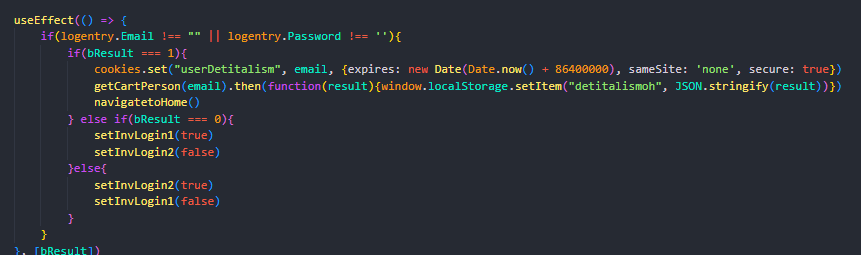
\includegraphics[width=0.9\linewidth]{images/CWE472-unsafe-LoginPage.png}
  \caption{CWE-472: Versão Insegura: LoginPage (app/src/Components/Pages/LoginPage.js)}
  \label{fig:cwe472-unsafe-loginpage}
\end{figure}
\begin{figure}[H]
  \centering
  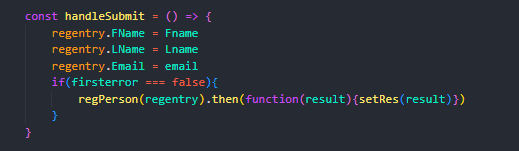
\includegraphics[width=0.8\linewidth]{images/CWE472-unsafe-RegisterPage.png}
  \caption{CWE-472: Versão Insegura: RegisterPage (app/src/Components/Pages/RegisterPage.js)}
  \label{fig:cwe472-unsafe-registerpage}
\end{figure}

\subsubsection{Correcção (app\_sec):}
Aplicando a função representada na figura \ref{fig:cwe472-safe-functionvalidinput} na LoginPage (figura\ref{fig:cwe472-safe-loginpage}) e na RegisterPage(figura\ref{fig:cwe472-safe-registerpage}) exerce-se a validação de valores de entrada.
\begin{figure}[H]
  \centering
  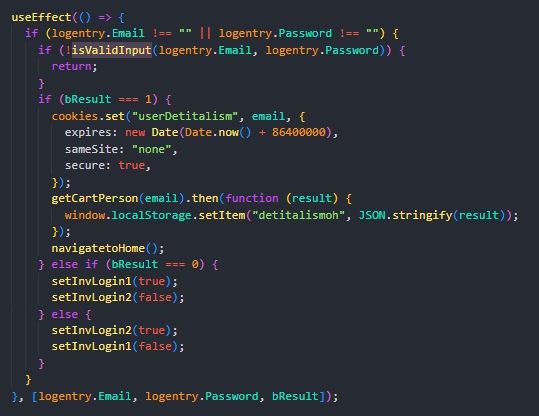
\includegraphics[width=0.8\linewidth]{images/CWE472-safe-LoginPage.png}
  \caption{CWE-472: Versão Segura: LoginPage (app\_sec/src/Components/Pages/LoginPage.js)}
  \label{fig:cwe472-safe-loginpage}
\end{figure}
\begin{figure}[H]
  \centering
  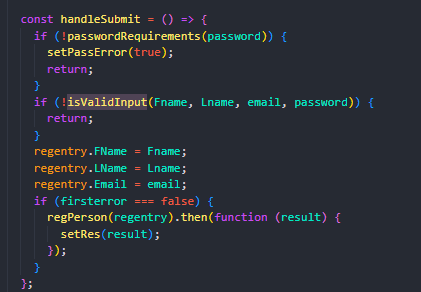
\includegraphics[width=0.8\linewidth]{images/CWE472-safe-RegisterPage.png}
  \caption{CWE-472: Versão Segura: RegisterPage (app\_sec/src/Components/Pages/RegisterPage.js)}
  \label{fig:cwe472-safe-registerpage}
\end{figure}
\begin{figure}[H]
  \centering
  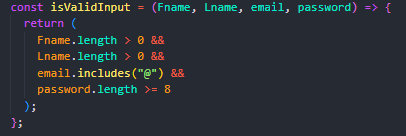
\includegraphics[width=0.8\linewidth]{images/CWE472-safe-functionValidInput.png}
  \caption{CWE-472: Versão Segura: função presente na LoginPage e na RegisterPage}
  \label{fig:cwe472-safe-functionvalidinput}
\end{figure}
%
%
%%%%%%%%%%%%%%%%%%%%%%%%%%%%%%%%%%%%%%%%%%%
\section{CWE-521: Weak Password Requirements}
\label{sec.cwe521}

A vulnerabilidade CWE-521, refere-se a requisitos de password fracos. Ocorre quando não são impostos os requisitos de segurança adequados para as passwords dos utilizadores. Pode resultar em passwords facilmente descobertas, comprometendo a segurança geral da aplicação e podendo expor os dados dos utilizadores. 

Para mitigar esta vulnerabilidade, é crucial implementar políticas para passwords robustas que exijam alguma complexidade das mesmas, incluindo uma combinação de caracteres alfanuméricos, símbolos especiais e letras maiúsculas e minúsculas. Além disso, é importante impor limites de comprimento e garantir que as senhas não sejam facilmente previsíveis ou baseadas em informações pessoais identificáveis.

\subsubsection{Demonstração e Impacto (app)}
Como se pode verificar a partir da figura, o registo de uma entidade não pressupõe qualquer tipo de requerimento de segurança sobre a password, deixando assim, a aplicação vulnerável a partir das entidades cujas passwords não sejam seguras.
\begin{figure}[H]
  \centering
  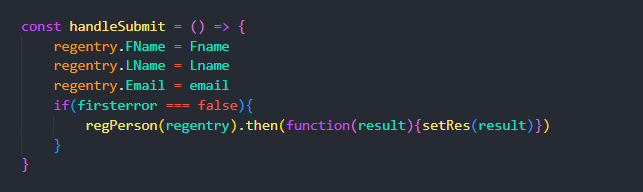
\includegraphics[width=16cm]{images/CWE521-unsafe.png}
  \caption{CWE-521: Exemplo 1 - Versão Insegura: RegisterPage (app/src/Components/Pages/RegisterPage.js)}
  \label{fig:cwe521-unsafe}
\end{figure}
\subsubsection{Correcção (app\_sec):}
A criação de uma função que garante que a password cumpre todos os requisitos no registo de uma conta assegurou a mitigação da vulnerabilidade.
Essa função pode ser vista na figura \ref{fig:cwe521-safe-registerpage2}.
\begin{figure}[H]
  \centering
    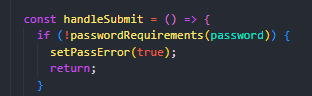
\includegraphics[width=0.8\linewidth]{images/CWE521-safe-RegisterPage1.png}
    \caption{CWE-521: Versão Segura: RegisterPage (http://localhost:3000/Register)}
    \label{fig:cwe521-safe-registerpage1}
\end{figure}
\begin{figure}[H]
  \centering
    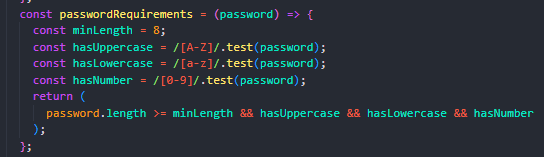
\includegraphics[width=0.8\linewidth]{images/CWE521-safe-RegisterPage2.png}
    \caption{CWE-521: Versão Segura: LoginPage  (http://localhost:3000/Login)}
    \label{fig:cwe521-safe-registerpage2}
\end{figure}

%
%
%%%%%%%%%%%%%%%%%%%%%%%%%%%%%%%%%%%%%%%%%%%
\section{CWE-541: Inclusion of Sensitive Information in an Include File}
\label{sec.cwe541}
Quando informações críticas (sensíveis) são inadvertidamente expostas devido à sua inclusão em arquivos (em forma de comentário, por exemplo) que não são adequadamente protegidos, pode criar riscos significativos, uma vez que estes arquivos podem ser acedidos por atacantes. Se as informações sensíveis não forem devidamente protegidas, um atacante com acesso a esses arquivos pode usá-las para fins maliciosos como exploração de vulnerabilidades reveladas ou até obter acesso não autorizado a dados confidenciais. \\
\subsubsection{Demonstração e Impacto (app)}
No decorrer do desenvolvimento da app.py (insegura), efectuámos diversos comentários sobre vulnerabilidades presentes no código. Este comentário podem ser usados por um atacante, facilitando a sua visão sobre a aplicação e a sua consequente exploração das vulnerabilidades incorrectamente indicadas. Seguidamente nas Figuras \ref{fig:cwe541-ex1} e \ref{fig:cwe541-ex2}, apresentamos dois exemplos deste problema na nossa base de dados insegura (app.py):

\begin{figure}[H]
  \centering
  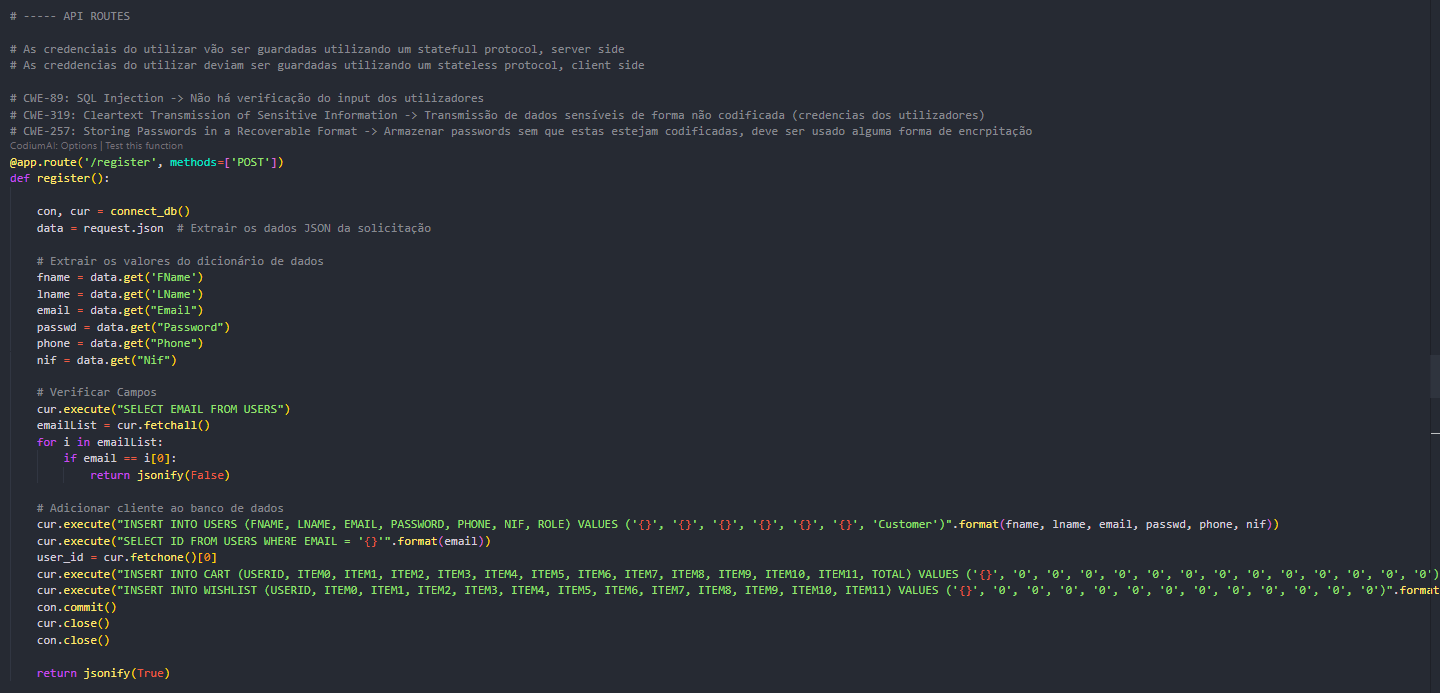
\includegraphics[width=16cm]{images/CWE-541-EX1.png}
  \caption{CWE-541: Exemplo 1 - Versão Insegura: Base de Dados (app.py)}
  \label{fig:cwe541-ex1}
\end{figure}

\begin{figure}[H]
  \centering
  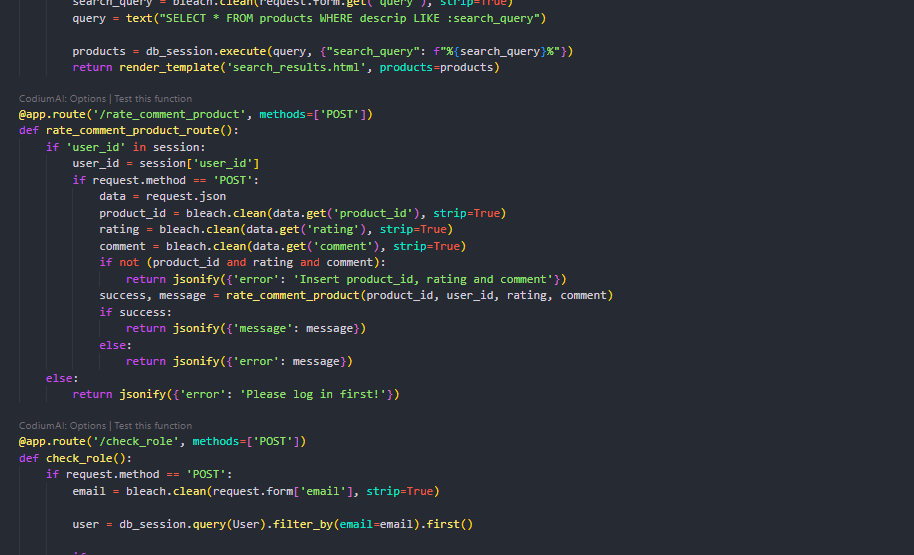
\includegraphics[width=16cm]{images/CWE-541-EX2.png}
  \caption{CWE-541: Exemplo 2 - Versão Insegura: Base de Dados (app.py)}
  \label{fig:cwe541-ex2}
\end{figure}

\subsubsection{Correcção (app\_sec):}
A remoção de comentários sensíveis (neste caso em específico sobre vulnerabilidades) resolve este problema. Devem ser apenas usados comentários de natureza relevante para os programadores sendo que a informação relativa a potenciais vulnerabilidades deve ser documentada em locais protegidos e acessíveis apenas por programadores da aplicação. 

\begin{figure}[H]
  \centering
  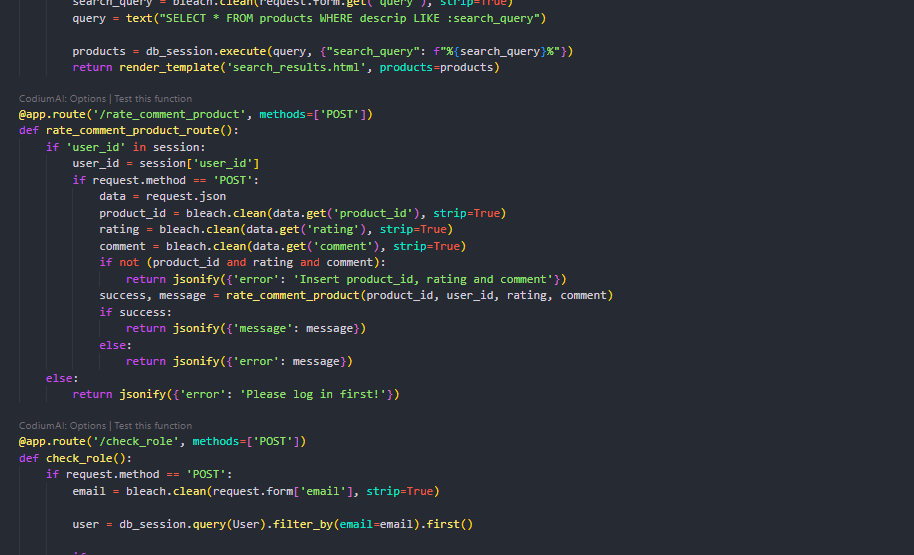
\includegraphics[width=16cm]{images/CWE-541-EX2.png}
  \caption{CWE-541: Exemplo 2 - Versão Segura: Base de Dados (app\_sec.py)}
  \label{fig:cwe541-ex2}
\end{figure}
%
%
%%%%%%%%%%%%%%%%%%%%%%%%%%%%%%%%%%%%%%%%%%%
\section{CWE-549: Missing Password Field Masking}
\label{sec.cwe549}
Campos de dados sensíveis, como passwords, em interfaces de utilizador devem ser "mascarados" durante a entrada de dados, para ocultar os caracteres enquanto o campo é preenchido pelo utilizador.É uma prática comum que envolve a substituição dos caracteres do campo por símbolos, como asteriscos ou pontos. \\ 
A ausência desta medida de segurança pode resultar em riscos de segurança, não protegendo visualmente os caracteres secretos, ficando expostos a qualquer pessoa que esteja próximo ou que esteja a monotorizar a interface gráfica (GUI) de forma ilegal, facilitando assim o acesso indevido a contas de utilizador e/ou roubo de informações sensíveis. \\

\subsubsection{Demonstração e Impacto (app)}
Na app insegura, nenhum dos dados sensíveis está mascarado de modo a garantir a anonimidade desses dados. Isto é evidente nas figuras  \ref{fig:cwe549-unsafe-register} e \ref{fig:cwe549-unsafe-login} abaixo.

\begin{figure}[H]
  \centering
  \begin{minipage}{0.45\textwidth}
    \centering
    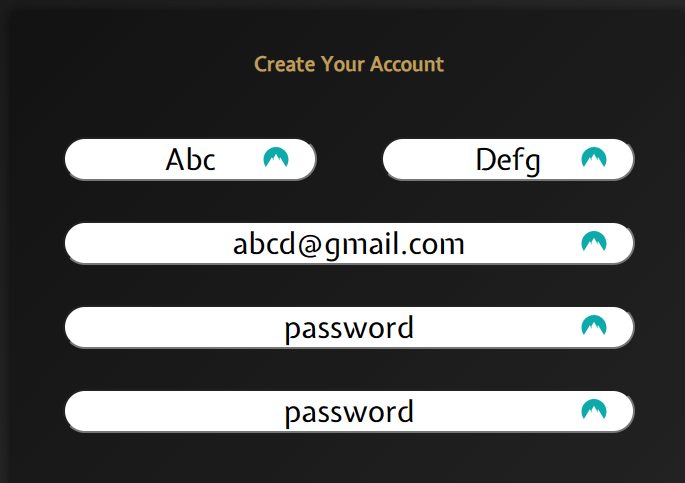
\includegraphics[width=0.8\linewidth]{images/CWE549-unsafe-register.png}
    \caption{CWE-549: Versão Insegura: RegisterPage (http://localhost:3000/Register)}
    \label{fig:cwe549-unsafe-register}
  \end{minipage}\hfill
  \begin{minipage}{0.45\textwidth}
    \centering
    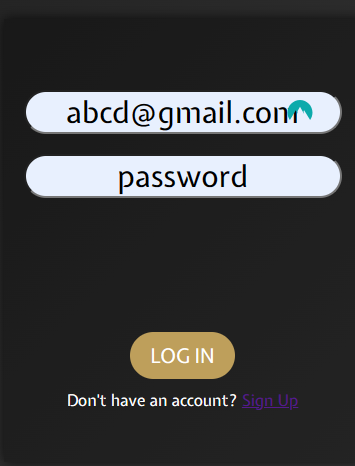
\includegraphics[width=0.8\linewidth]{images/CWE549-unsafe-login.png}
    \caption{CWE-549: Versão Insegura: LoginPage  (http://localhost:3000/Login)}
    \label{fig:cwe549-unsafe-login}
  \end{minipage}
\end{figure}

\begin{figure}[H]
  \centering
  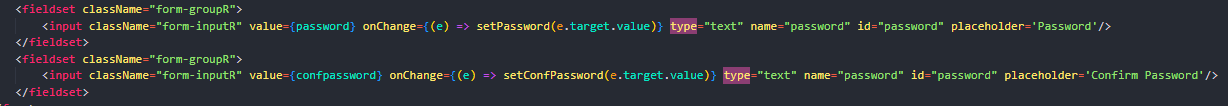
\includegraphics[width=16cm]{images/CWE549-unsafe-RegisterPage.png}
  \caption{CWE-549: Versão Insegura: RegisterPage (app/src/Components/Pages/RegisterPage.js)}
  \label{fig:cwe549-unsafe-registerpage}
\end{figure}

\begin{figure}[H]
  \centering
  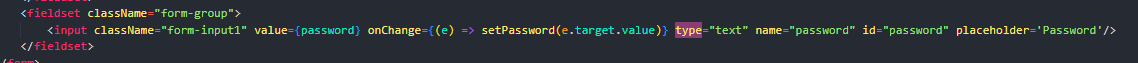
\includegraphics[width=16cm]{images/CWE549-unsafe-LoginPage.png}
  \caption{CWE-549: Versão Insegura: LoginPage (app/src/Components/Pages/LoginPage.js)}
  \label{fig:cwe549-unsafe-loginpage}
\end{figure}
\subsubsection{Correcção (app\_sec):}
Ao alterar o atributo type da password para "password", como demonstra nas figuras \ref{fig:cwe549-safe-registerpage} e \ref{fig:cwe549-safe-loginpage}, os caracteres da password passam a ser representados por pontos, mascarando-a. Figuras \ref{fig:cwe549-safe-register} e \ref{fig:cwe549-safe-login}

\begin{figure}[H]
  \centering
  \begin{minipage}{0.45\textwidth}
    \centering
    \includegraphics[width=0.8\linewidth]{images/CWE549-safe-register.png}
    \caption{CWE-549: Versão Segura: RegisterPage (http://localhost:3000/Register)}
    \label{fig:cwe549-safe-register}
  \end{minipage}\hfill
  \begin{minipage}{0.45\textwidth}
    \centering
    \includegraphics[width=0.8\linewidth]{images/CWE549-safe-login.png}
    \caption{CWE-549: Versão Segura: LoginPage  (http://localhost:3000/Login)}
    \label{fig:cwe549-safe-login}
  \end{minipage}
\end{figure}

\begin{figure}[H]
  \centering
  \includegraphics[width=16cm]{images/CWE549-safe-RegisterPage.png}
  \caption{CWE-549: Versão Segura: RegisterPage (app\_sec/src/Components/Pages/RegisterPage.js)}
  \label{fig:cwe549-safe-registerpage}
\end{figure}

\begin{figure}[H]
  \centering
  \includegraphics[width=16cm]{images/CWE549-safe-LoginPage.png}
  \caption{CWE-549: Versão Segura: LoginPage (app\_sec/src/Components/Pages/LoginPage.js)}
  \label{fig:cwe549-safe-loginpage}
\end{figure}
%
%
%%%%%%%%%%%%%%%%%%%%%%%%%%%%%%%%%%%%%%%%%%%
\section{CWE-620: Unverified Password Change}
A vulnerabilidade CWE-620 refere-se à capacidade de alterar a password do utilizador sem ser necessário fornecer a password antiga. Como consequência, na eventualidade de um atacante conseguir acessar a conta, este poderá alterar a password sem dificuldade e negar o acesso à conta ao utilizador.
\label{sec.cwe620}
\subsubsection{Demonstração e Impacto (app)}
Como é demonstrado nas figuras \ref{fig:cwe620-unsafe-changepasspage} e \ref{fig:cwe620-unsafe-app}, para a mudança de password apenas é necessário introduzir a nova password pretendida, tornando-se assim uma ação de fácil execução
\begin{figure}[H]
   \centering
    \includegraphics[width=0.7\linewidth]{images/CWE620-unsafe-ChangePassPage.png}
    \caption{CWE620: Versão Insegura: ChangePassPage }(app/src/Components/Pages/ChangePassPage.js)%7D
    \label{fig:cwe620-unsafe-changepasspage}
\end{figure}
\begin{figure}[H]
  \centering
    \includegraphics[width=0.7\linewidth]{images/CWE620-unsafe-app.png}
    \caption{CWE620: Versão Insegura: app  }(app/src/backend/app.py)%7D
    \label{fig:cwe620-unsafe-app}
\end{figure}


\subsubsection{Correcção (app\_sec):}
Para garantir que a password não é alterada por algum atacante, a alteração da password requer a introdução da password antiga. Para tal, adicionámos a variável \textit{oldpass}, figura \ref{fig:cwe620-safe-changepasspage} que será necessária para a operação em causa, figura \ref{fig:cwe620-safe-app} .
\begin{figure}[H]
\centering
    \includegraphics[width=0.7\linewidth]{images/CWE620-safe-ChangePassPage.png}
    \caption{CWE620: Versão Insegura: ChangePassPage }(app\_sec/src/Components/Pages/ChangePassPage.js)%7D
    \label{fig:cwe620-safe-changepasspage}
\end{figure}
\begin{figure}[H]
\centering
    \includegraphics[width=0.7\linewidth]{images/CWE620-safe-app_sec.png}
    \caption{CWE620: Versão Insegura: app  }(app\_sec/src/backend/app\_sec.py)%7D
    \label{fig:cwe620-safe-app}
\end{figure}

%%%%%%%%%%%%%%%%%%%%%%%%%%%%%%%%%%%%%%%%%%%

\section{CWE-710: Improper Adherence to Coding Standards e CWE-1006: Bad Coding Practices}
\label{sec.cwe710}
\label{sec.cwe1006}
Uma solução de software deve aderir rigorosamente às diretrizes e práticas do paradigma de programação do seu domínio, a fim de prevenir potenciais vulnerabilidades. 

\subsubsection{Demonstração e Impacto (app)}
A base de dados insegura, foi criada num único ficheiro \textit{app.py} (sendo não modelar) e verifica-se um grande agrupamento de código que pode tornar as suas leitura, compreensão e/ou correcção complexas, tanto para o programador como para o analista de segurança responsável por auditorias subsequentes, tal como demonstrado nas Figuras seguintes:

\begin{figure}[H]
  \centering
  \includegraphics[width=16cm]{images/CWE-710-EX1.png}
  \caption{CWE: 710 - Exemplo 1 - Versão insegura (app)}
  \label{fig:fig:cwe710-ex1}
\end{figure}

\begin{figure}[H]
  \centering
  \includegraphics[width=16cm]{images/CWE-710-EX2.png}
  \caption{CWE: 710 - Exemplo 2 - Versão insegura (app)}
  \label{fig:fig:cwe710-ex2}
\end{figure}

\subsubsection{Correcção (app\_sec):}
Para corrigir o problema de boas práticas e modelaridade presentes na aplicação insegura, esta foi restruturada em diversos modulos, dividindo o seu código em "blocos" o que, com uso de boas práticas, torna toda a organização, leitura, compreensão e correcção mais simples e eficiente do ponto de vista do programador ou analista.

\begin{figure}[H]
  \centering
  \includegraphics[width=5cm]{images/CWE-710-Modular.png}
  \caption{CWE: 710 - Versão Segura (backend modular)}
  \label{fig:fig:cwe710-ex2}
\end{figure}
%
%
%%%%%%%%%%%%%%%%%%%%%%%%%%%%%%%%%%%%%%%%%%%
\section{Vulnerabilidade subtil - Light Analysis Failure}
\label{sec.subtil}
Existe uma vulnerabilidade subtil que pode não ser detectada por \textit{"light analysis"}. Esta encontra-se implementada na função \textbf{\textit{new\_customer}}.

\subsubsection{Demonstração e Impacto (app)}
Esta função permite a um atacante efectuar um registo múltiplas vezes usando as mesmas credenciais, alterando letras maiúsculas e minúsculas, tal como demonstrado na Figura \ref{fig:subtil}

\begin{figure}[H]
  \centering
  \includegraphics[width=16cm]{images/Subtil.png}
  \caption{Vulnerabilidade subtil - Base de Dados(app.py)}
  \label{fig:subtil}
\end{figure}

\subsubsection{Correcção (app\_sec):}
Para corrigir, tal como demonstrado na Figura \ref{fig:corr-subtil}, a função foi rescrita em SQLAlchemy fazendo uso de confirmações de \textit{"password matching"} e do método \textit{"filter\_by"} para efectuar a \textit{query} de forma \textit{case-sensitive}, corrigindo efectivamente o problema descrito.

\begin{figure}[H]
  \centering
  \includegraphics[width=16cm]{images/Correcção-Subtil.png}
  \caption{Vulnerabilidade subtil corrigida: Base de Dados(app\_sec.py)}
  \label{fig:corr-subtil}
\end{figure}
%
%
%
%%%%%%%%%%%%%%%%%%%%%%%%%%%%%%%%%%%%%%%%%%%%%%%%%%%%%%%%%
%%%%%%%%%%%%%%%%%%%%%%%%%%%%%%%%%%%%%%%%%%%%%%%%%%%%%%%%%
%%%%%CONCLUSÃO
%
\chapter*{Conclusão:}
\label{chap.conclusão}
\lhead{Conclusão}
No decorrer deste projecto, foi efectuada uma análise abrangente do ciclo de vida de desenvolvimento da aplicação, partindo de uma implementação insegura até alcançar uma versão segura e corrigida. Este processo destacou a importância crítica da cibersegurança e das práticas adequadas de programação no desenvolvimento de soluções adequadas para \textit{deployment} na Web. \\

Foi possível efectuar com sucesso todos os objectivos espectados:
    \begin{itemize}
        \item Na versão inicial da solução aplicacional foram implementadas, identificadas, testadas e analisadas diversas \acf{cwe} que simulam uma solução com riscos de segurança significativos para o sistema e futuros utilizadores.
        \item  Posteriormente, dada a análise (auditoria) anteriormente efectuada, a solução insegura foi corrigida adequadamente tornando-a assim, mais segura.
    \end{itemize}

Este projecto ilustra claramente as consequências significativas no mundo real das práticas seguras de programação para aplicações e/ou soluções Web. A negligência em relação às boas práticas e segurança  pode resultar em violações de dados e privacidade, perdas financeiras, furto de identidade e danos à reputação de uma organização ou utilizador comum.
%
%%%%%%%%%%%%%%%%%%%%%%%%%%%%%%%%%%%%%%%%%%%%%%%%%%%%%%%%%
%%%%%CONTRIBUIÇÕES DE AUTORES:
% 
\chapter*{Contribuições dos Autores}

        Os autores responsáveis pela pesquisa e desenvolvimento do presente projecto, contribuiram de forma coletiva, refletindo-se diversidade de experiências, opiniões e competências que enriqueceram a abordagem ao mesmo. Este projecto pode ser visualizado na sua totalidade na página: \textbf{\url{https://github.com/detiuaveiro/1st-project-group_26}}. \\

        \textbf{Autores:}
        \begin{itemize}
            \item João Pedro Nunes Vieira, NºMec.: 50458
            \item José Miguel Guardado Silva, Nº Mec.: 103248
            \item Henrique Miguel Escudeiro Cruz, Nº Mec.: 103442
            \item Luís Manuel Trindade Diogo, Nº Mec.: 108668

        \begin{table}[H]
            \centering
            \caption{Contribuições dos Autores.}
            \small
            \begin{tabular}{|c|c|c|c|c|}\hline
                Contribuição & João Vieira & José Silva & Henrique Cruz & Luís Diogo  \\ 
                \hline
        	    Produção de Relatório (LaTex)                           & 25~\% & 25~\% & 25~\% & 25~\% \\
                Identificação e descrição de CWEs                       & 25~\% & 25~\% & 25~\% & 25~\% \\
                Desenvolvimento de Front-End inseguro (REACT)           & 0~\% & 50~\% & 0~\% & 50~\% \\
                Desenvolvimento de Front-End seguro (REACT)             & 0~\% & 50~\% & 0~\% & 50~\% \\
                Desenvolvimento de Back-End inseguro (SQLite e Flask)   & 50~\% & 0~\% & 50~\% & 0~\% \\
        	    Desenvolvimento de Back-End seguro (SQLAlchemy e Flask) & 50~\% & 0~\% & 50~\% & 0~\% \\
                Testes e Depuração                                      & 25~\% & 25~\% & 25~\% & 25~\% \\   
            \hline
            \end{tabular}
            \label{tab.contribuições}
        \end{table}	
        
        
        \end{itemize}

%
%%%%%%%%%%%%%%%%%%%%%%%%%%%%%%%%%%%%%%%%%%%%%%%%%%%%%%%%%
%%%%%BIBLIOGRAFIA:
%
\begin{thebibliography}{9}

\bibitem{thinkpython} 
Allen Downey
\textit{Think Python - How to Think Like a Computer Scientist}. |
Green Tea Press, 2nd Edition, Version 2.4.0, 2015

\bibitem{segredes} 
André Zúquete
\textit{Segurança em Redes Informáticas}. |
FCA - Editora de Informática LDA, 5th Edition, 2018

\bibitem{mitrepdf} 
The MITRE Corporation
\text{ https://cwe.mitre.org/data/published/cwe\_latest.pdf }. | \\
CWE - Version 4.13 - (2023-10-26), Copyright 2023, The MITRE Corporation

\bibitem{Wikipedia}
Wikipédia: Enciclopédia livre. |
\text{ pt.wikipedia.org, acedido 10/10/2023.}

\bibitem{sqlite}
SQLite Website. |
\text{ https://www.sqlite.org/docs.html, acedido 11/10/2021.}

\bibitem{sqlalchemy}
SQLAlchemy Website. |
\text{ https://docs.sqlalchemy.org/en/20/, acedido 11/10/2021.}

\bibitem{mitre}
MITRE: A Community-Developed List of Software and Hardware Weakness Types. |
\text{ https://cwe.mitre.org/index.html, acedido 16/10/2021.}

\end{thebibliography}
\end{document}